\documentclass[a4paper,12pt]{article}

\usepackage{graphicx}
\usepackage[usenames,dvipsnames]{xcolor}
\usepackage{tcolorbox}
\usepackage{tabularx}
\usepackage{array}
\usepackage{colortbl}
\tcbuselibrary{skins}
\usepackage{tablefootnote}
\usepackage[a4paper, total={6.5in, 8in}]{geometry}
\usepackage[backend=biber,style=numeric,citestyle=authortitle-ibid]{biblatex}
\usepackage{qrcode}
\usepackage{environ}
\usepackage{xcolor}
\usepackage[tikz]{bclogo}
\usepackage{tikz}
\usetikzlibrary{calc}
\usepackage[colorlinks=true,linkcolor=blue]{hyperref}
\usepackage[utf8]{inputenc}

% Steps
\usepackage{enumitem}
\newlist{steps}{enumerate}{1}
\setlist[steps, 1]{label = Step \arabic*:}

\newcolumntype{Y}{>{\raggedleft\arraybackslash}X}

\tcbset{tab1/.style={fonttitle=\bfseries\large,fontupper=\normalsize\sffamily,
colback=yellow!10!white,colframe=red!75!black,colbacktitle=Salmon!40!white,
coltitle=black,center title,freelance,frame code={
\foreach \n in {north east,north west,south east,south west}
{\path [fill=red!75!black] (interior.\n) circle (3mm); };},}}

\tcbset{tab2/.style={enhanced,fonttitle=\bfseries,fontupper=\normalsize\sffamily,
colback=yellow!10!white,colframe=red!50!black,colbacktitle=Salmon!40!white,
coltitle=black,center title}}

\newcounter{stepcounter}

\addbibresource{cite.bib} % include citation file

\begin{document}
\begin{titlepage}
    \centering 
    \vfill
    
\includegraphics[width=10cm]{ilri_logo.png}
    \vfill 
    {\bfseries\Large
        USER GUIDE\\
        FOR\\
        FEED FORMULATION APPLICATION\\
        \vskip2cm
    }   
    
    \vfill 
    \vfill 
    \vspace{50pt}
    \textbf{A comprehensive user manual for Feed Formulation App\\
			Addis Ababa, ETHIOPIA\\
			Version 1.0\\
			26/12/2023
		}
    
    \vfill
\end{titlepage}

\newpage

\tableofcontents
\newpage

\pagenumbering{arabic}

\section{Legend}
\begin{tcolorbox}[tab2,tabularx={X|Y|Y|Y|Y}]
\textbf{Name} & \textbf{Abbreviation} & \textbf{Unit}  & \textbf{Description} \\\hline
Dry matter & DM & \% &  The dry matter or dry weight is a measure of the mass of a completely dried substance.\footcite{enwiki:1178208071} \\\hline

Metabolizable Energy   & ME & kcal/kg 	&  \\\hline

Crude protein   	& CP	& \% 		&  \\\hline
Lysine   & Lys 		& \% 	&	\\\hline
Meth. +cystine   	& m+c 	& \% 		&  \\\hline
Methionine   		& Met 	& \% 		&  \\\hline
Ether extract   		& EE 	& \% 		&  \\\hline
Crude fiber   		& CF 	& \% 		&  \\\hline
Calcium & Ca 	& \% 		&  \\\hline
Phosphorus   		& P 	& \% 		&  \\\hline
\end{tcolorbox}

\section{Glossary}
\begin{tabular}{p{8cm}p{11cm}}
Ration &  \\
\\
Formulation &  \\
\\
Formula &  \\
\\
Grid Formulation &  \\
\\
Ingredients &  \\
\\
Ingredient Group &  \\
\\
Ingredient Composition &  \\
\\
Nutrient Group &  \\
\\
Nutrients &  \\
\\
Requirements &  \\
\\
Requirement Compostion &  \\
\\
Requirement Boundires & (Min \& Max)  \\
\\

\\

\end{tabular}

\newpage
\section{Introduction}
Feed Formula Application is dummy text


\NewEnviron{myremark}[1]
  {\par\medskip\noindent
  \begin{tikzpicture}
    \node[inner sep=0pt] (box) {\parbox[t]{.99\textwidth}{%
      \begin{minipage}{.3\textwidth}
      \centering\tikz[scale=5]\node[scale=3,rotate=30]{\bclampe};
      \end{minipage}%
      \begin{minipage}{.65\textwidth}
      \textbf{#1}\par\smallskip
      \BODY
      \end{minipage}\hfill}%
    };
    \draw[red!75!black,line width=3pt] 
      ( $ (box.north east) + (-5pt,3pt) $ ) -- ( $ (box.north east) + (0,3pt) $ ) -- ( $ (box.south east) + (0,-3pt) $ ) -- + (-5pt,0);
    \draw[red!75!black,line width=3pt] 
      ( $ (box.north west) + (5pt,3pt) $ ) -- ( $ (box.north west) + (0,3pt) $ ) -- ( $ (box.south west) + (0,-3pt) $ ) -- + (5pt,0);
  \end{tikzpicture}\par\medskip%
}

\begin{myremark}{To Access The App}\label{visite_site}
\vspace{10px}
Scan the QR Code or go to: \href{http://172.27.1.72:3000/}{http://172.27.1.72:3000/}

\vspace{20px}

\quad
\qrcode[height=1in]{http://172.27.1.72:3000?qrcode=true}
\end{myremark}

\newpage

\setcounter{stepcounter}{1}

\paragraph{\arabic{stepcounter}.}Access the website refre to \ref{visite_site}.
If you already have an account login by following  \hyperref[sec:login]{section \ref{sec:login}}.

\stepcounter{stepcounter}
\paragraph{\arabic{stepcounter}.} Enter the required information (Full name, Email address \& message), Click "Submit" and wait for email response.
\begin{figure}[h!]
  	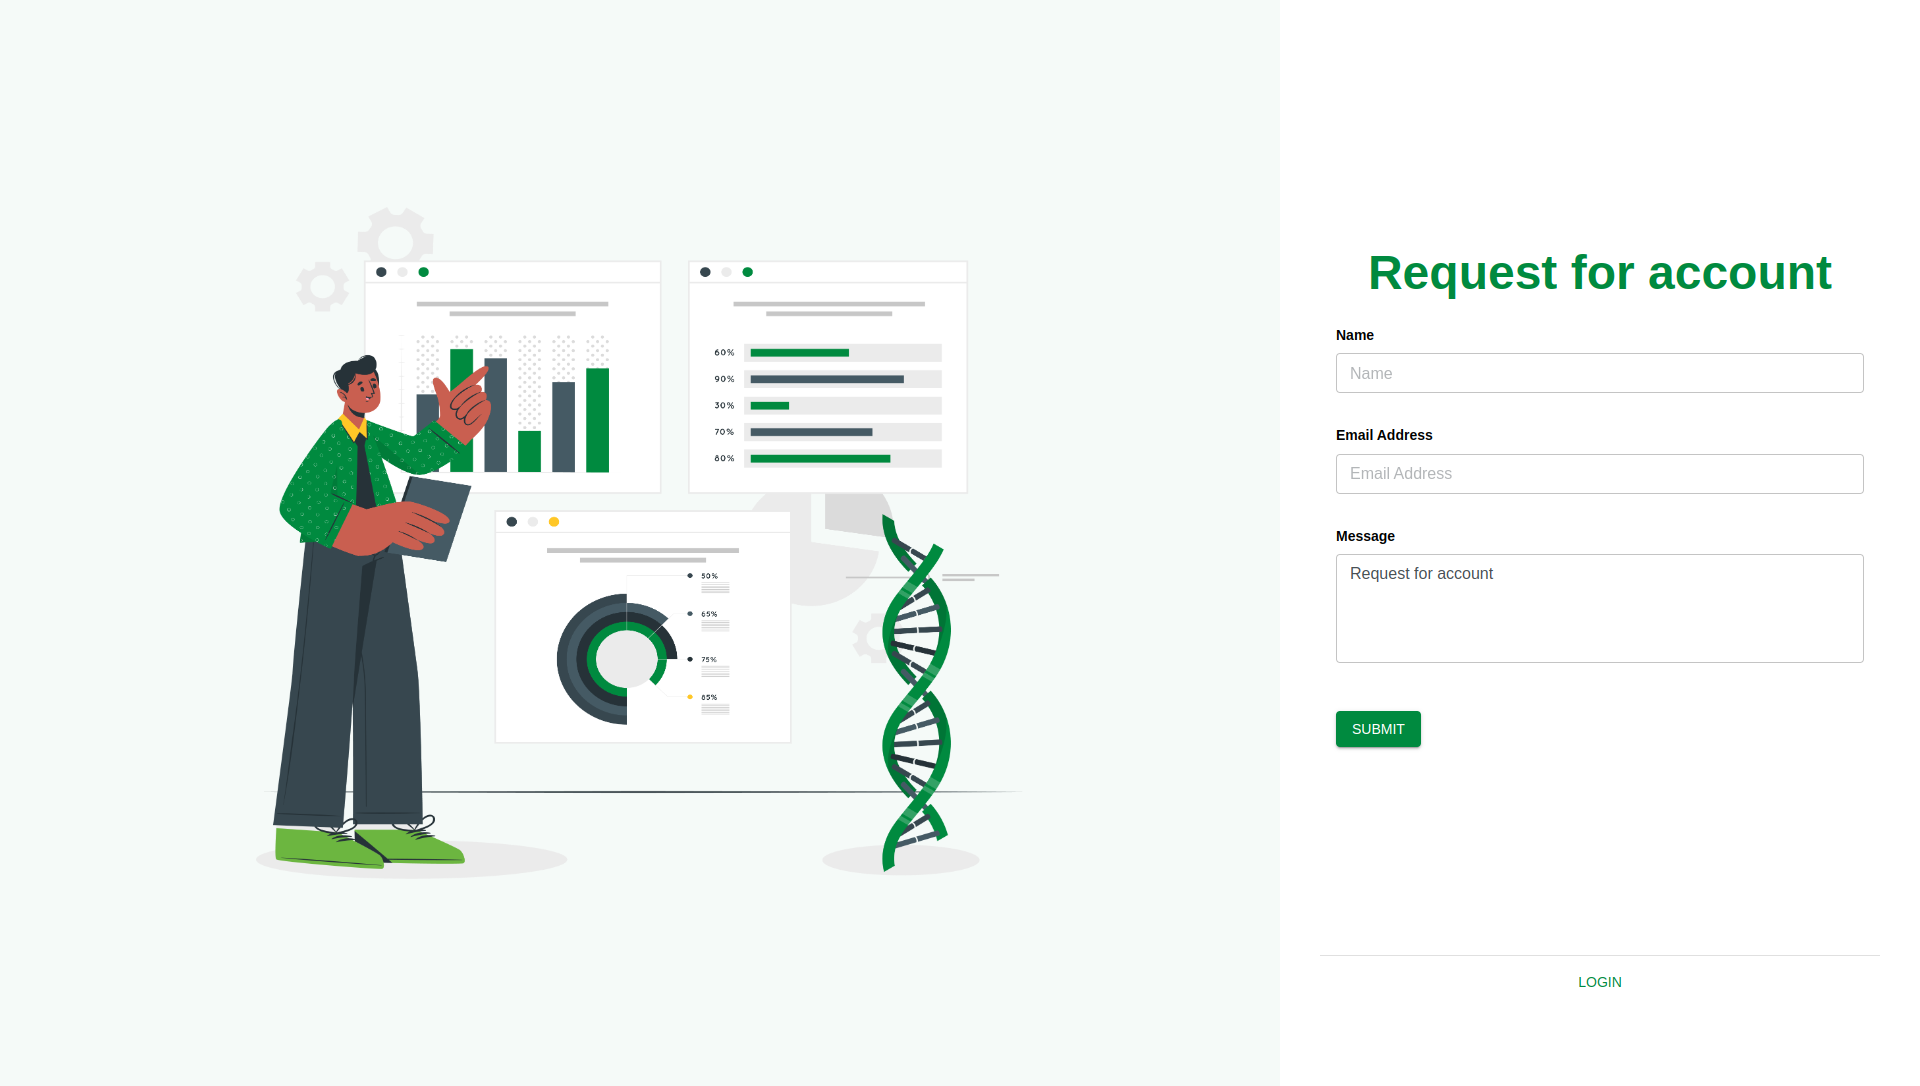
\includegraphics[width=15cm]{screenshots/sign_up_page.png}
  	\caption{Sign up page}
  	\label{fig:sign_up_page}
\end{figure}

\stepcounter{stepcounter}
\paragraph{\arabic{stepcounter}.} Go to your email inbox to create new account.

\begin{myremark}{Haven't recived invitation email?}\label{visite_site}
You will only recive an invitation email address, if the request is approved by admins. For further detail contact support \hyperref[sec:login]{support address \ref{sec:login}}
\end{myremark}

Click "Join" and you will be redirect to account creation page.
\begin{figure}[h!]
  	
\includegraphics[width=15cm]{screenshots/verify_invitation_page.png}
  	\caption{Verify Invitation Page}
  	\label{fig:verify_invitation_page}
\end{figure}
Enter the required fields and click \textcolor{ForestGreen}{"CREATE NEW ACCOUNT"}.

\newpage
\section{Login}\label{sec:login}
\begin{figure}[h!]
  	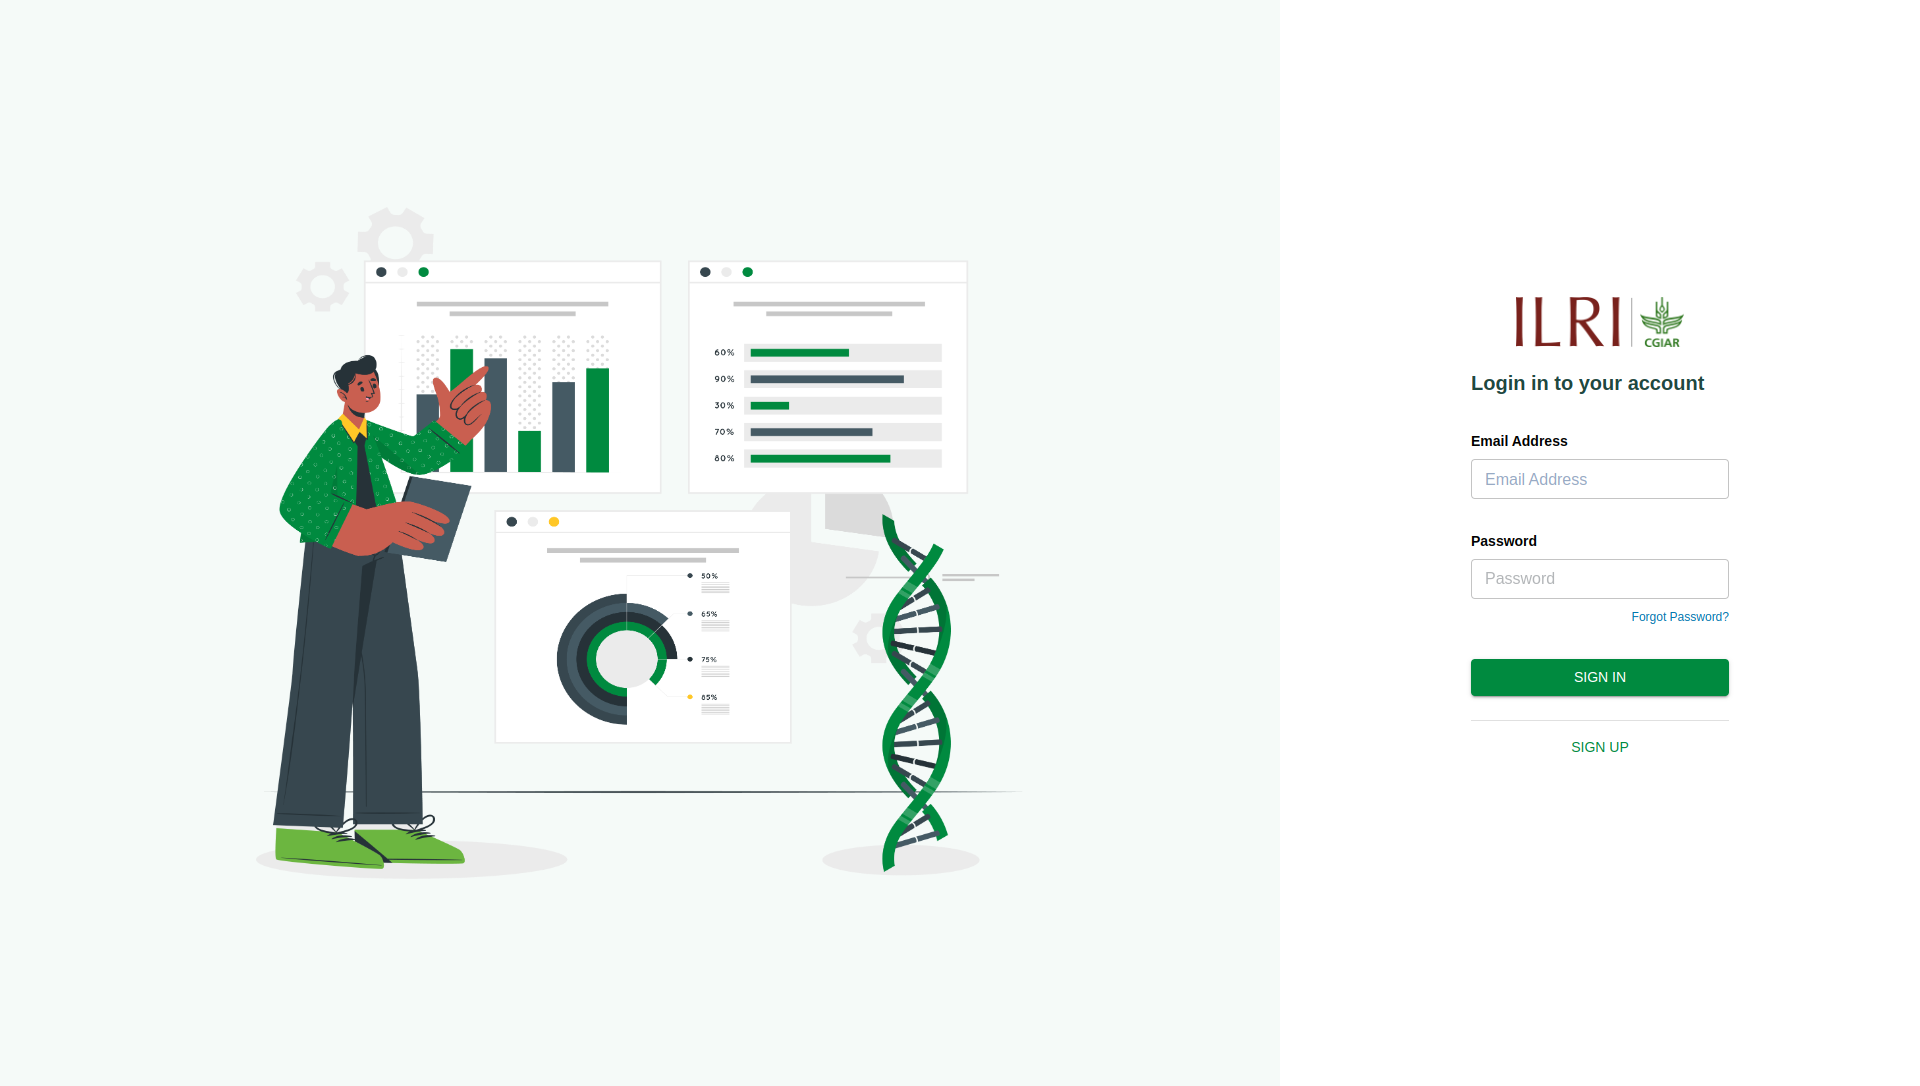
\includegraphics[width=15cm]{screenshots/login_page.png}
  	\caption{Login Page}
  	\label{fig:login_page}
\end{figure}

\newpage
\section{Forgot Password}
\begin{figure}[h!]
  	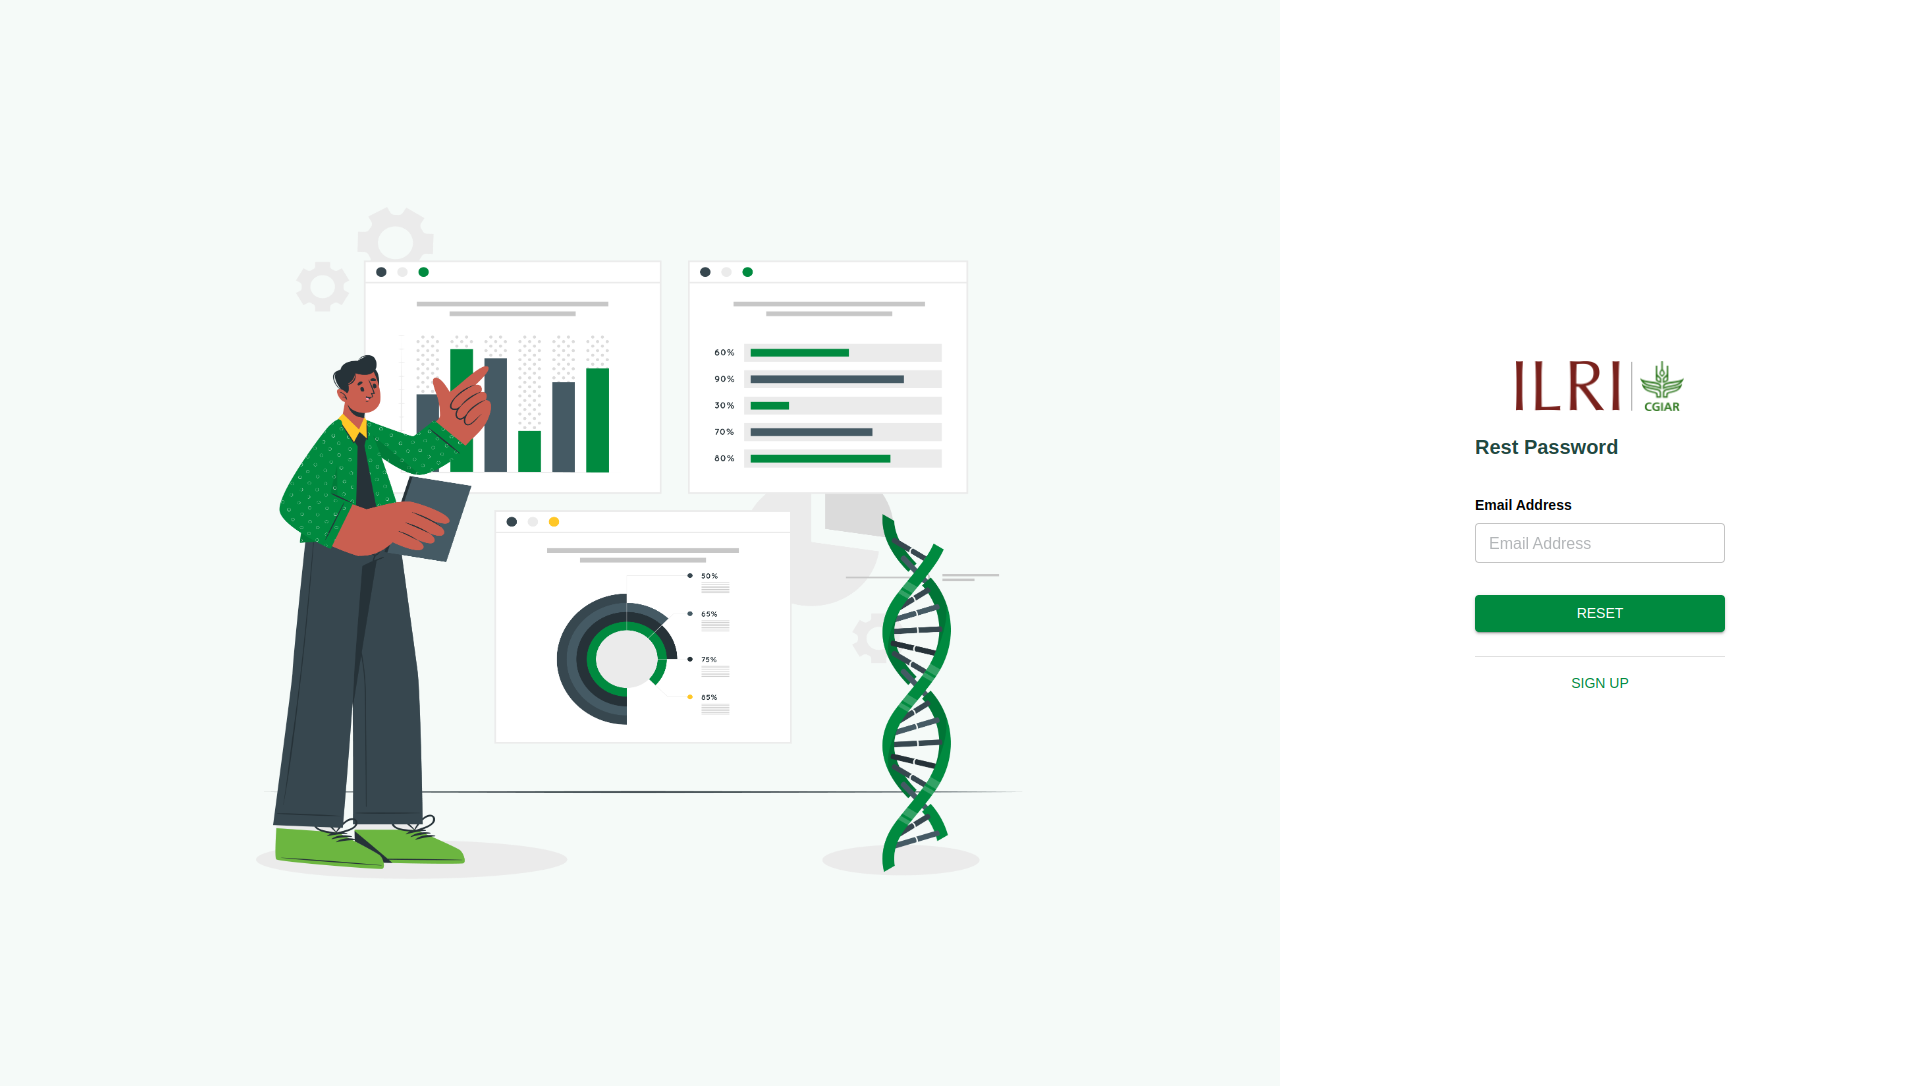
\includegraphics[width=15cm]{screenshots/forgot_password_page.png}
  	\caption{Forgot Password Page}
  	\label{fig:forgot_password_page}
\end{figure}

\newpage
\section{First View}\label{sec:first_view}
\begin{figure}[h!]
  	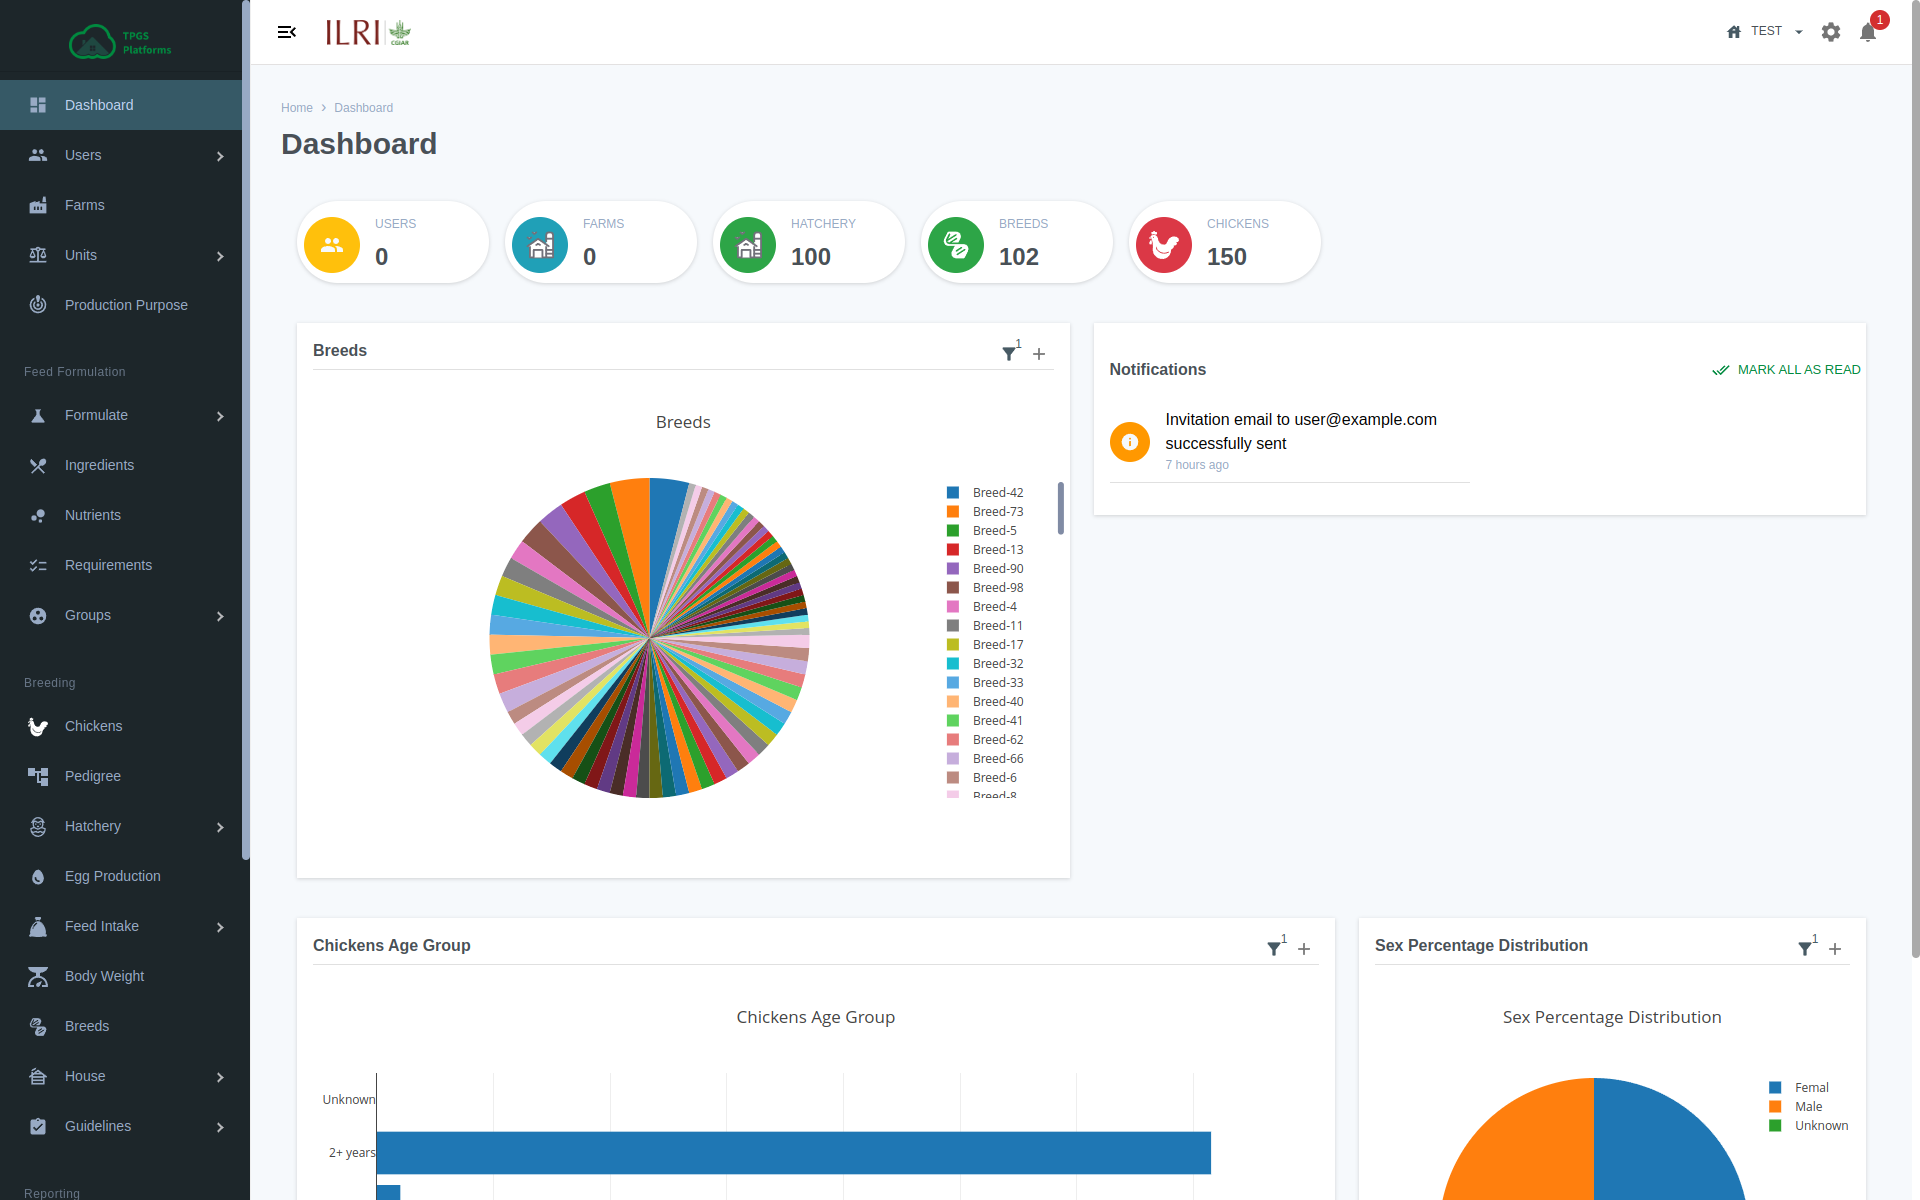
\includegraphics[width=15cm]{screenshots/dashboard_page.png}
  	\caption{Dashboard Page}
  	\label{fig:dashboard_page}
\end{figure}

\newpage
\section{Manage Farm}\label{sec:farm}
Switch farm either by going to \textcolor{ForestGreen}{Farms} menu or by click on top right farm menu.
\begin{figure}[h!]
  	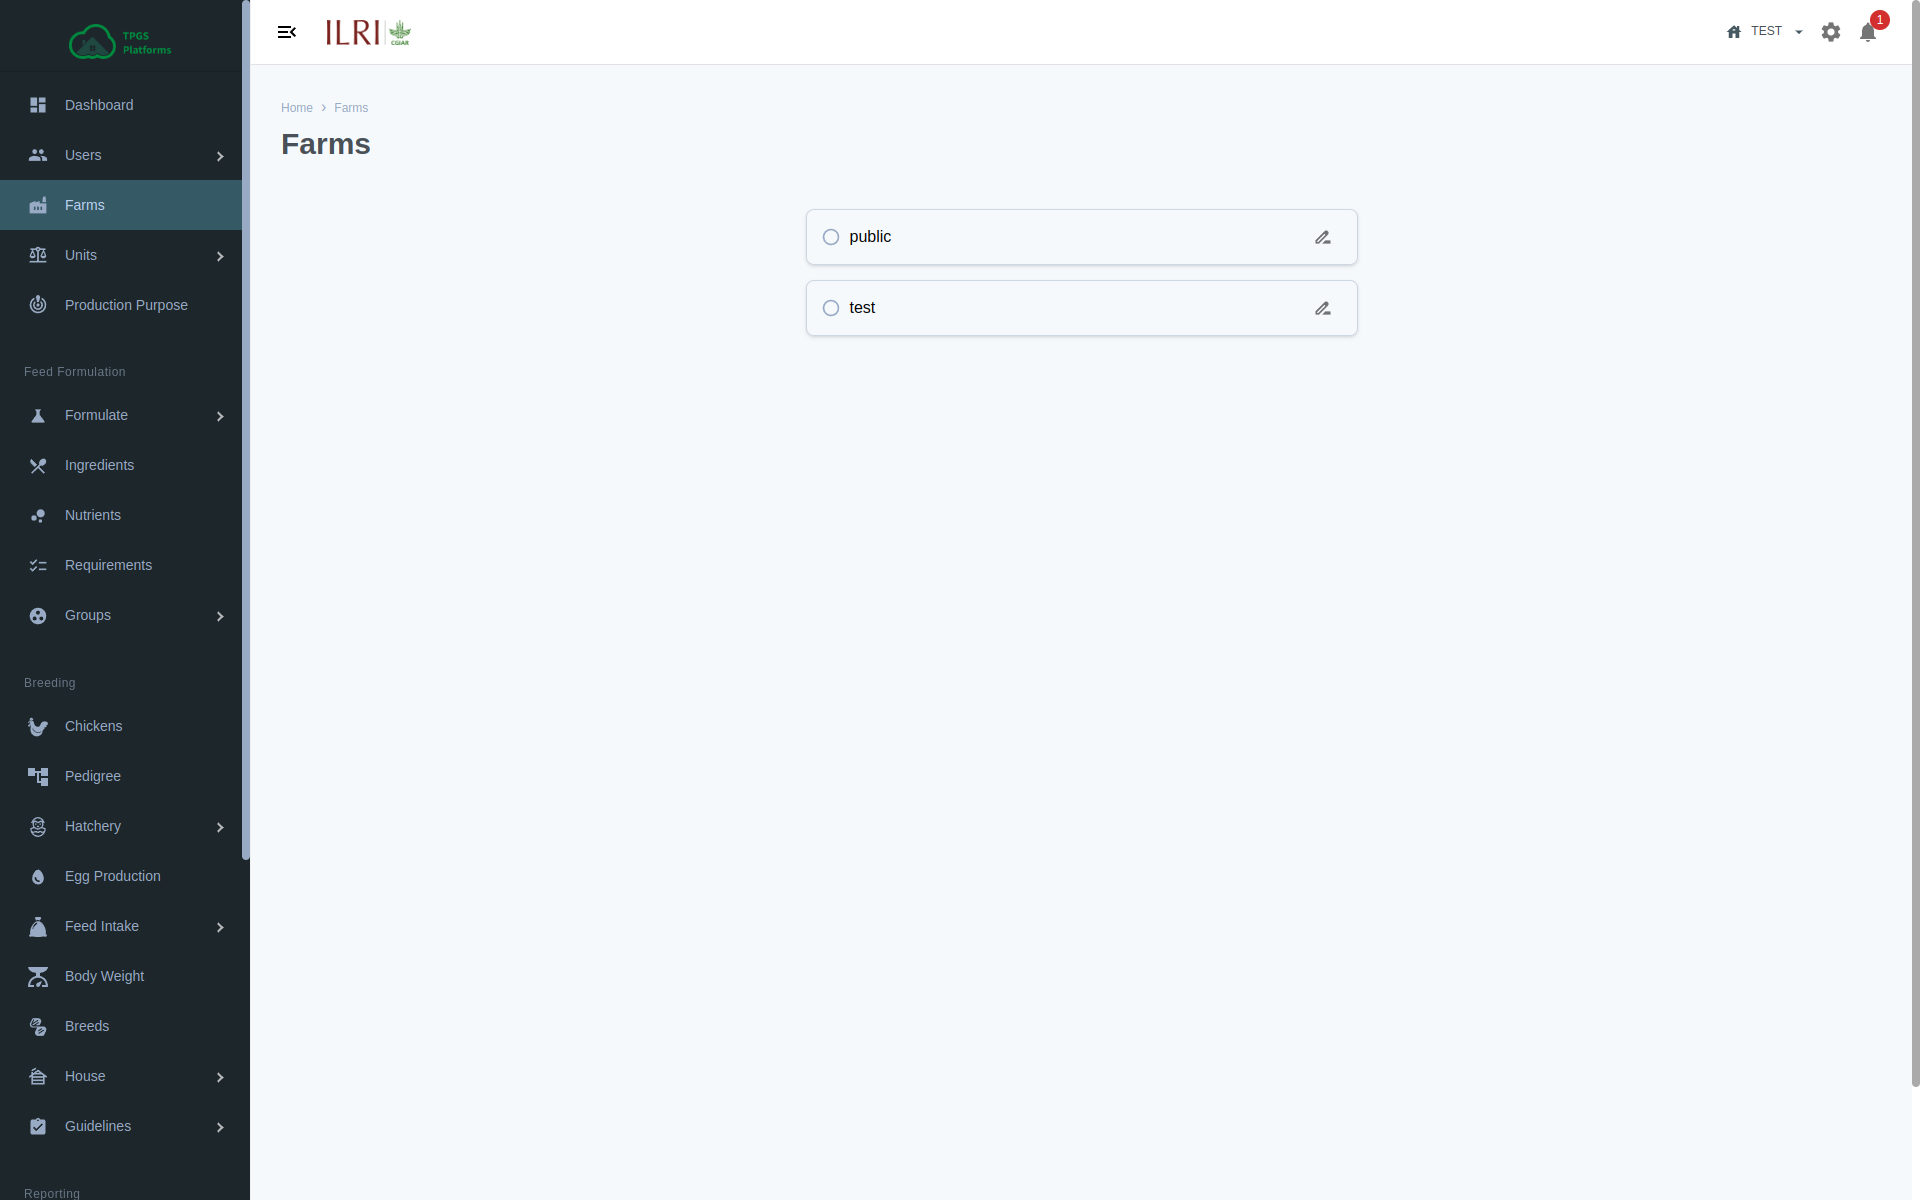
\includegraphics[width=15cm]{screenshots/farm_page.png}
  	\caption{Switch Farm}
  	\label{fig:farm_page}
\end{figure}

\newpage
\section{Unit}\label{sec:unit}

\subsection{View Unit List}\label{sec:unit_list}
\setcounter{stepcounter}{1}
\paragraph{\arabic{stepcounter}.}Click on \textcolor{ForestGreen}{"Unit"}
\begin{figure}[h!]
  	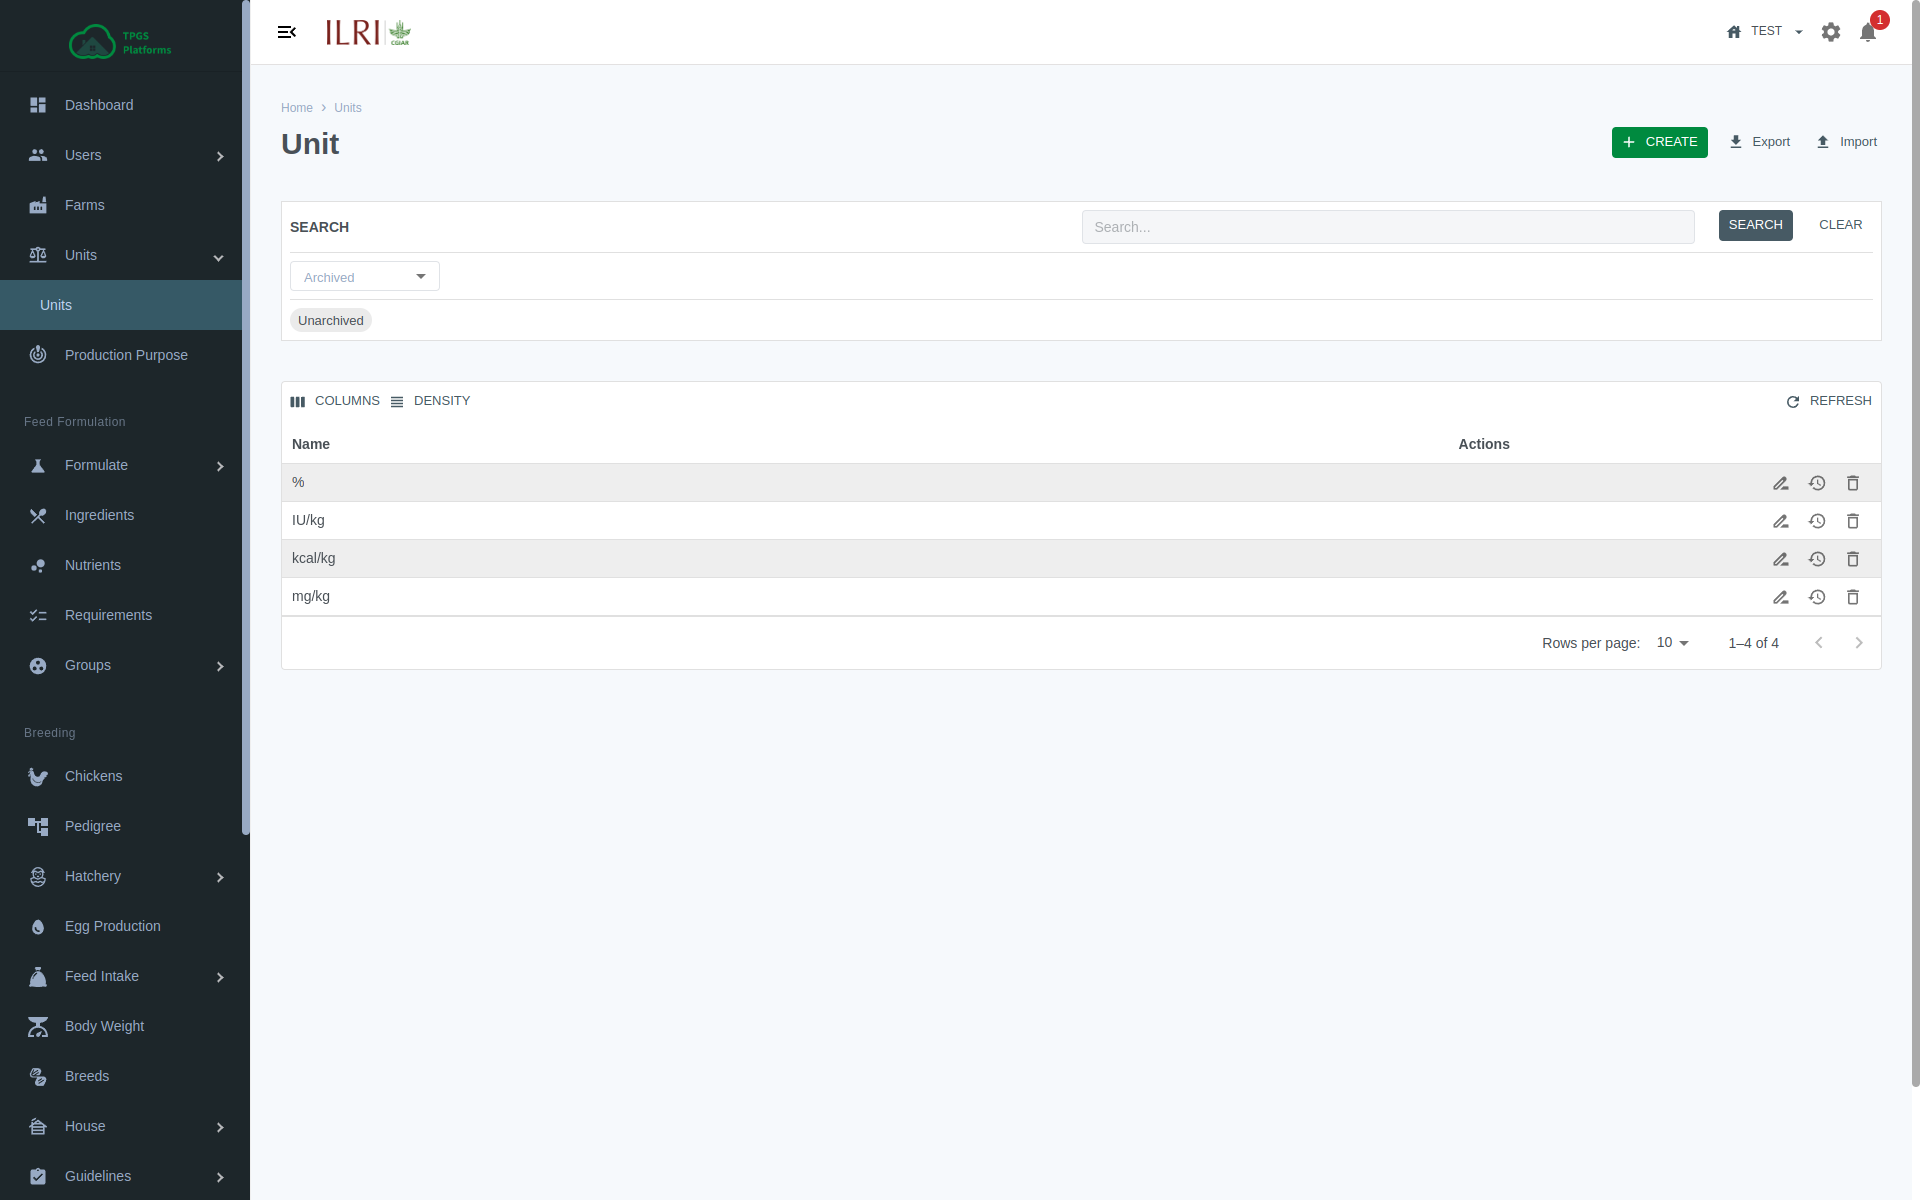
\includegraphics[width=15cm]{screenshots/unit_list_page.png}
  	\caption{Unit List}
  	\label{fig:unit_list_page}
\end{figure}

\subsection{Archive Records}\label{sec:unit_list_archived}
\setcounter{stepcounter}{1}
\paragraph{\arabic{stepcounter}.}On filter section filter the records by archive.

\subsection{Create new Unit}\label{sec:unit_create}
\setcounter{stepcounter}{1}
\paragraph{\arabic{stepcounter}.}To create new unit click on \textcolor{ForestGreen}{"Create"} Refer \hyperref[fig:unit_list_page]{Figure \ref{fig:unit_list_page}}
\begin{figure}[h!]
  	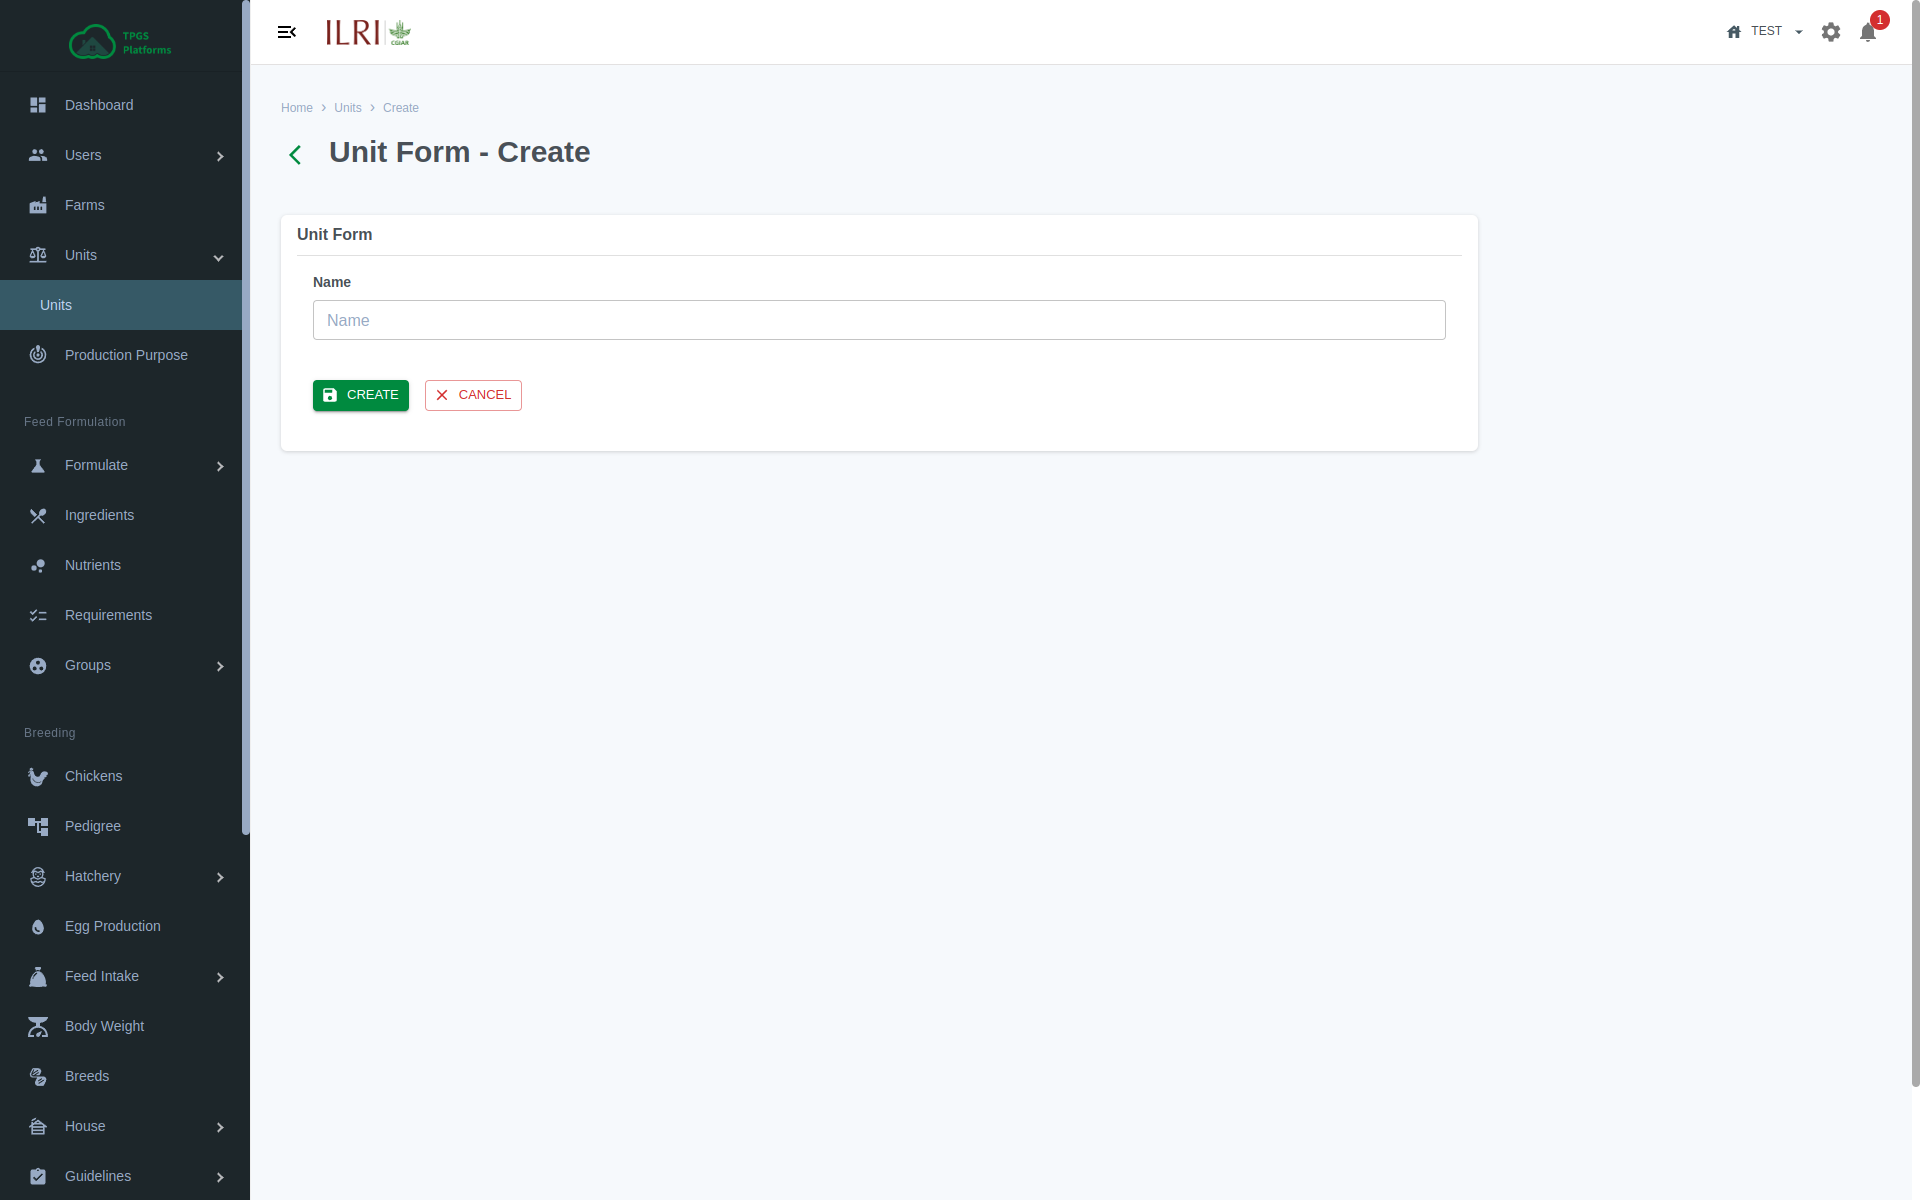
\includegraphics[width=15cm]{screenshots/unit_create_page.png}
  	\caption{Create new Nutrient Group}
  	\label{fig:unit_create_page}
\end{figure}
And click \textcolor{ForestGreen}{"CREATE"}, you will be redirect to  \hyperref[sec:unit_list]{Section \ref{sec:unit_list}}

\subsection{Edit Unit}\label{sec:unit_edit}
\setcounter{stepcounter}{1}
\paragraph{\arabic{stepcounter}.}Go to the Unit\hyperref[sec:unit_list]{Refer to Section \ref{sec:unit_list}}, then click on Pencil icon and it will redirect to the \hyperref[fig:unit_edit_page]{Figure \ref{fig:unit_edit_page}}.
\begin{figure}[h!]
  	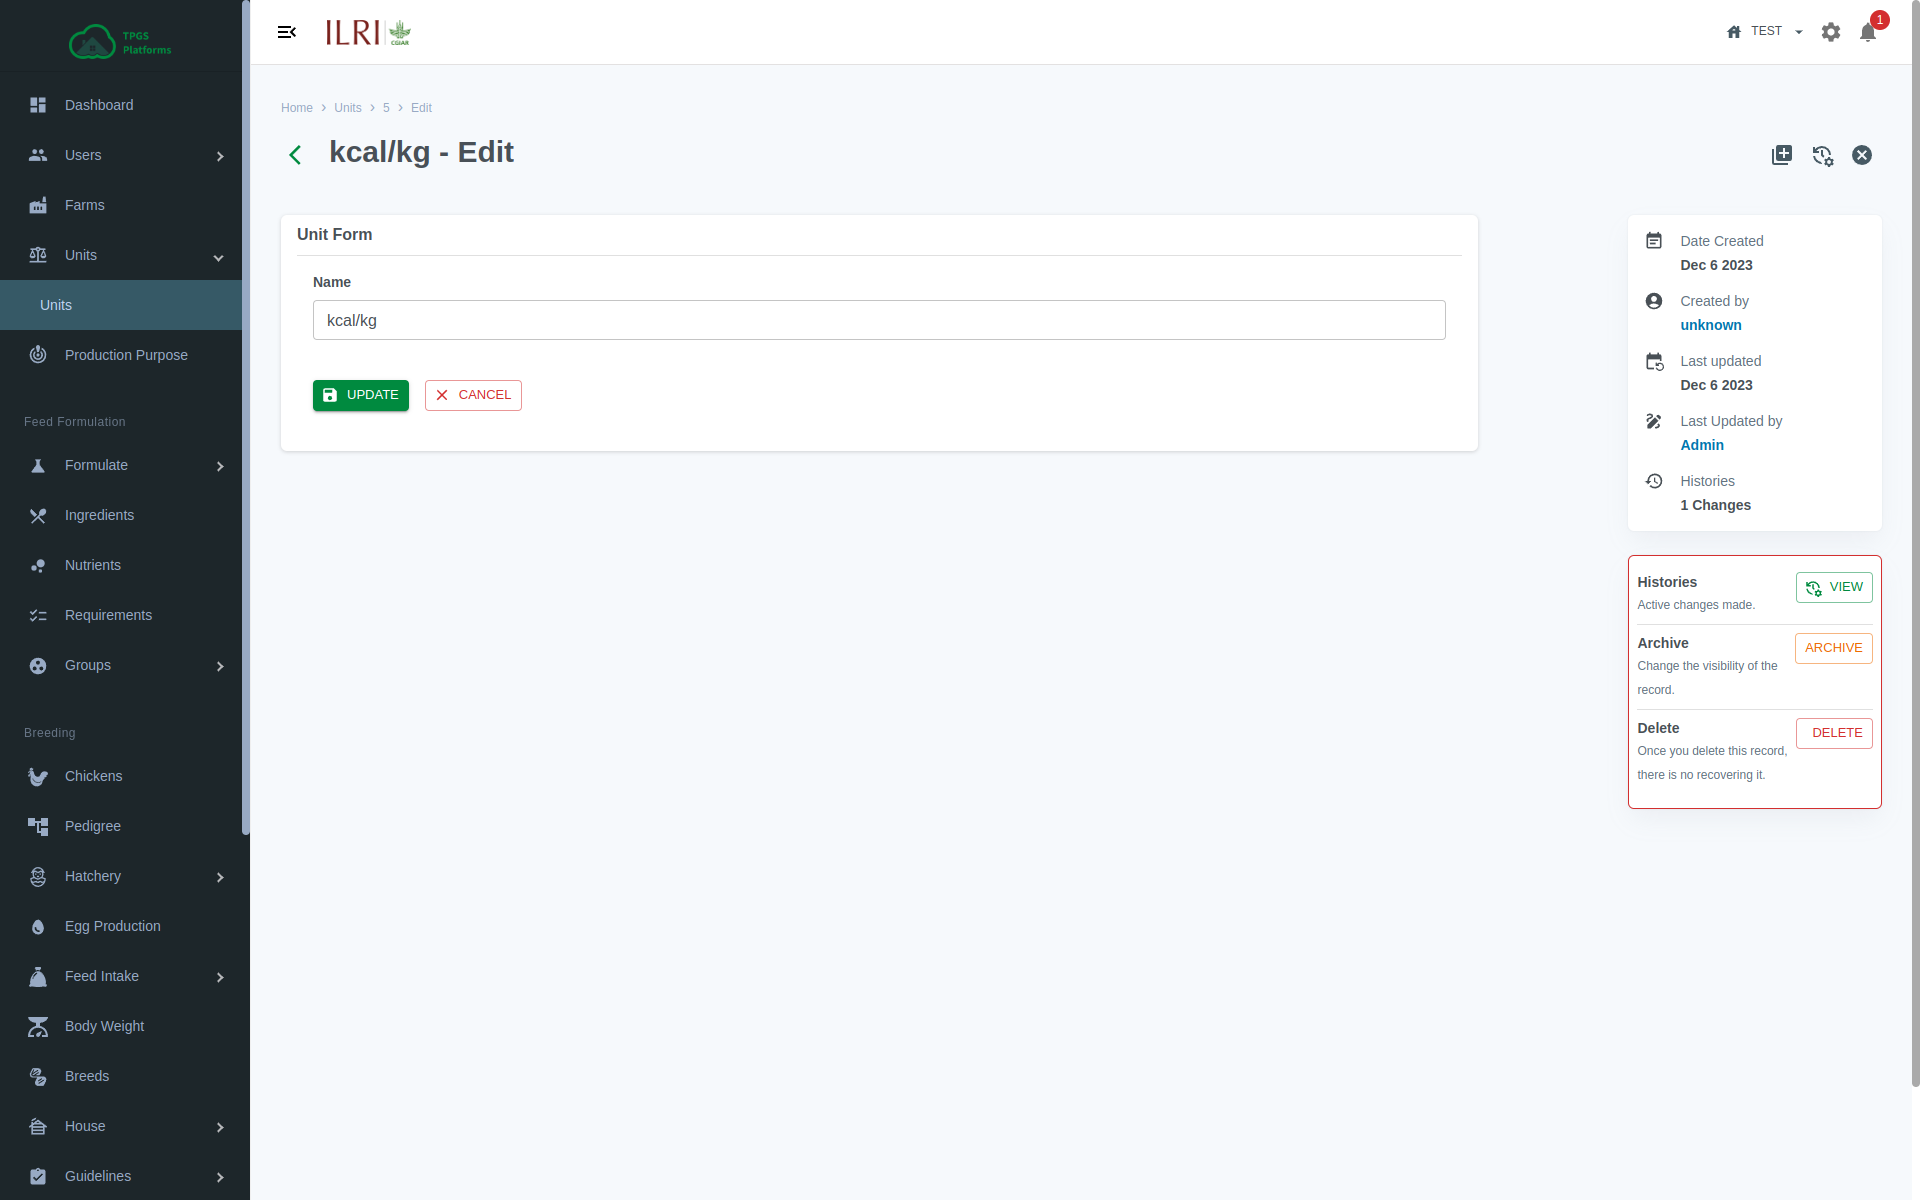
\includegraphics[width=15cm]{screenshots/unit_edit_page.png}
  	\caption{Edit Unit}
  	\label{fig:unit_edit_page}
\end{figure}

\subsection{Delete Unit}
\setcounter{stepcounter}{1}
\paragraph{\arabic{stepcounter}.}Go to the edit Unit \hyperref[sec:unit_edit]{Refer to Section \ref{sec:unit_edit}}.

\paragraph{\arabic{stepcounter}.}To archive the record click on \textcolor{ForestGreen}{"Archive"}. If you want to bring back the record/unarchive follow the step under \hyperref[sec:unit_list_archived]{Section  \ref{sec:unit_list_archived}}, and click on \textcolor{ForestGreen}{"UnArchive"}


\paragraph{\arabic{stepcounter}.}To permanently delete the record click on \textcolor{ForestGreen}{"Delete"}.

\begin{figure}[h!]
  	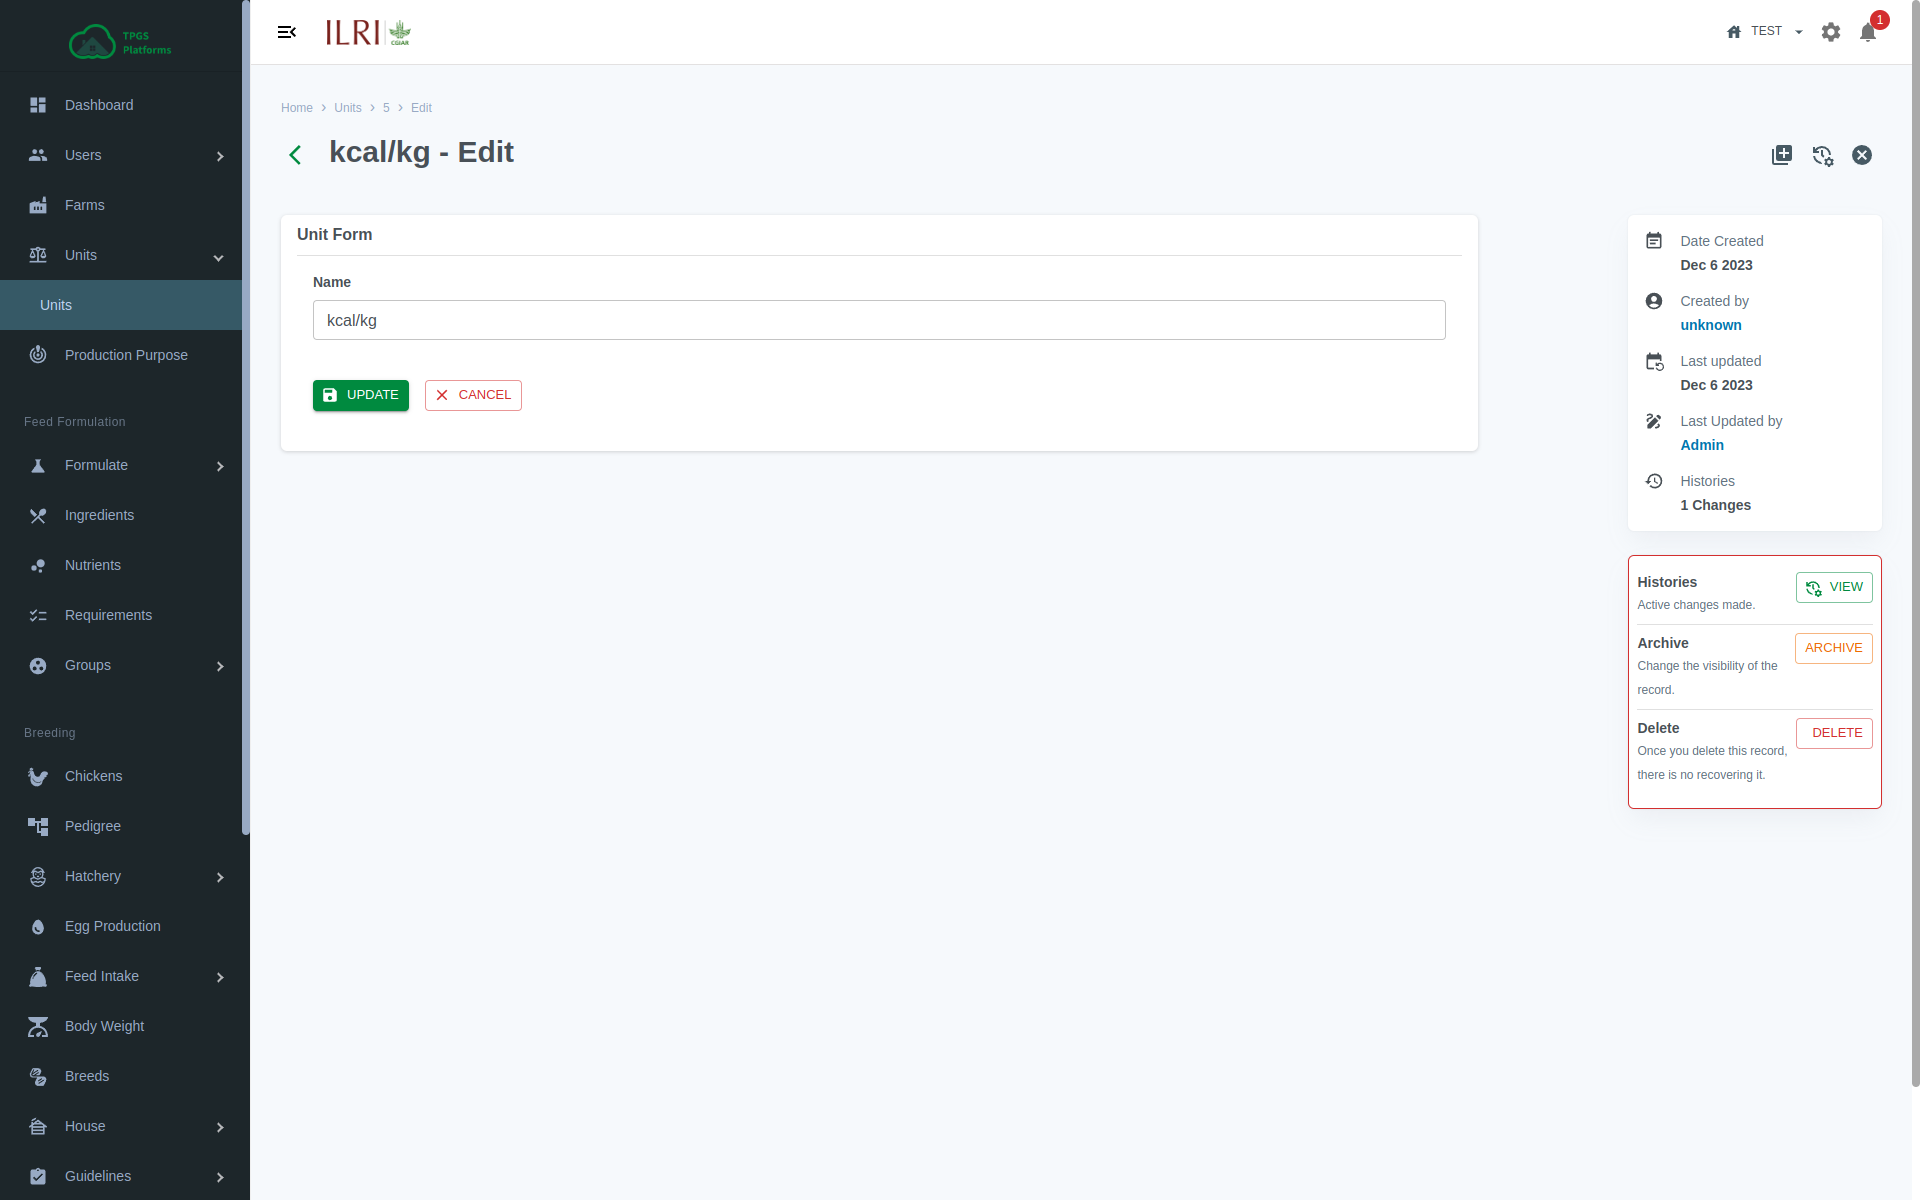
\includegraphics[width=15cm]{screenshots/unit_edit_page.png}
  	\caption{Edit Unit}
  	\label{fig:unit_edit_page}
\end{figure}

\newpage
\section{Production Purposes}\label{sec:production_purpose}

\subsection{Production Purpose List}\label{sec:production_purpose_list}
\setcounter{stepcounter}{1}
\paragraph{\arabic{stepcounter}.}Access Production Purposes list by clicking on \textcolor{ForestGreen}{"Production Purpose"} from left 
\paragraph{\arabic{stepcounter}.}Expand \textcolor{ForestGreen}{"Group"} menu and click on \textcolor{ForestGreen}{"Nutrient Group"}
\begin{figure}[h!]
  	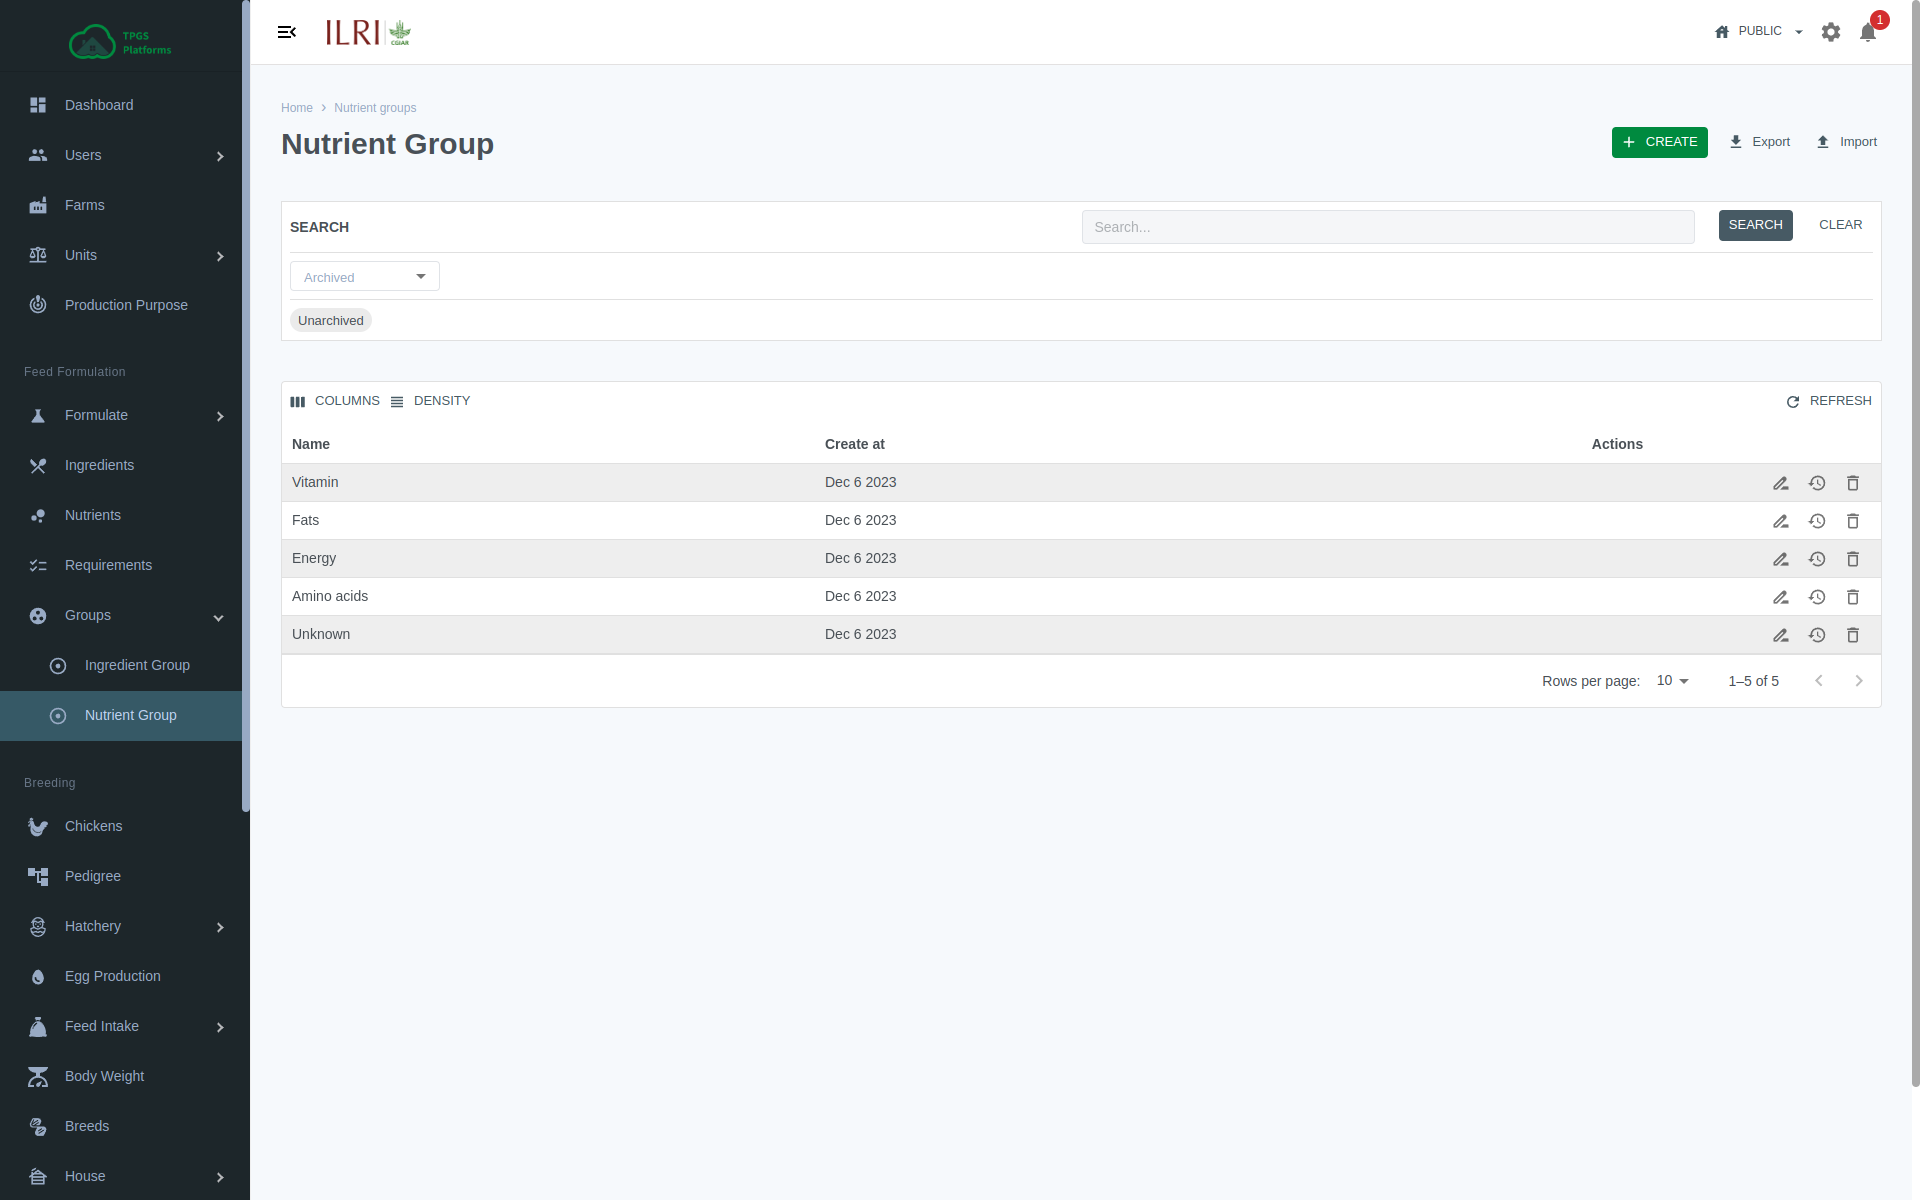
\includegraphics[width=15cm]{screenshots/nutrient_group_list_page.png}
  	\caption{Nutrient Group List}
  	\label{fig:nutrient_group_list_page}
\end{figure}

\subsection{Archive Records}\label{sec:nutrient_group_list_archived}
\setcounter{stepcounter}{1}
\paragraph{\arabic{stepcounter}.}On filter section filter the records by archive.

\subsection{Create new Nutrient Group}\label{sec:nutrient_group_create}
\setcounter{stepcounter}{1}
\paragraph{\arabic{stepcounter}.}To create new nutrient group click on \textcolor{ForestGreen}{"Create"} \hyperref[fig:nutrient_group_list_page]{Refer from nutrient list Figure \ref{fig:nutrient_group_list_page}}
\begin{figure}[h!]
  	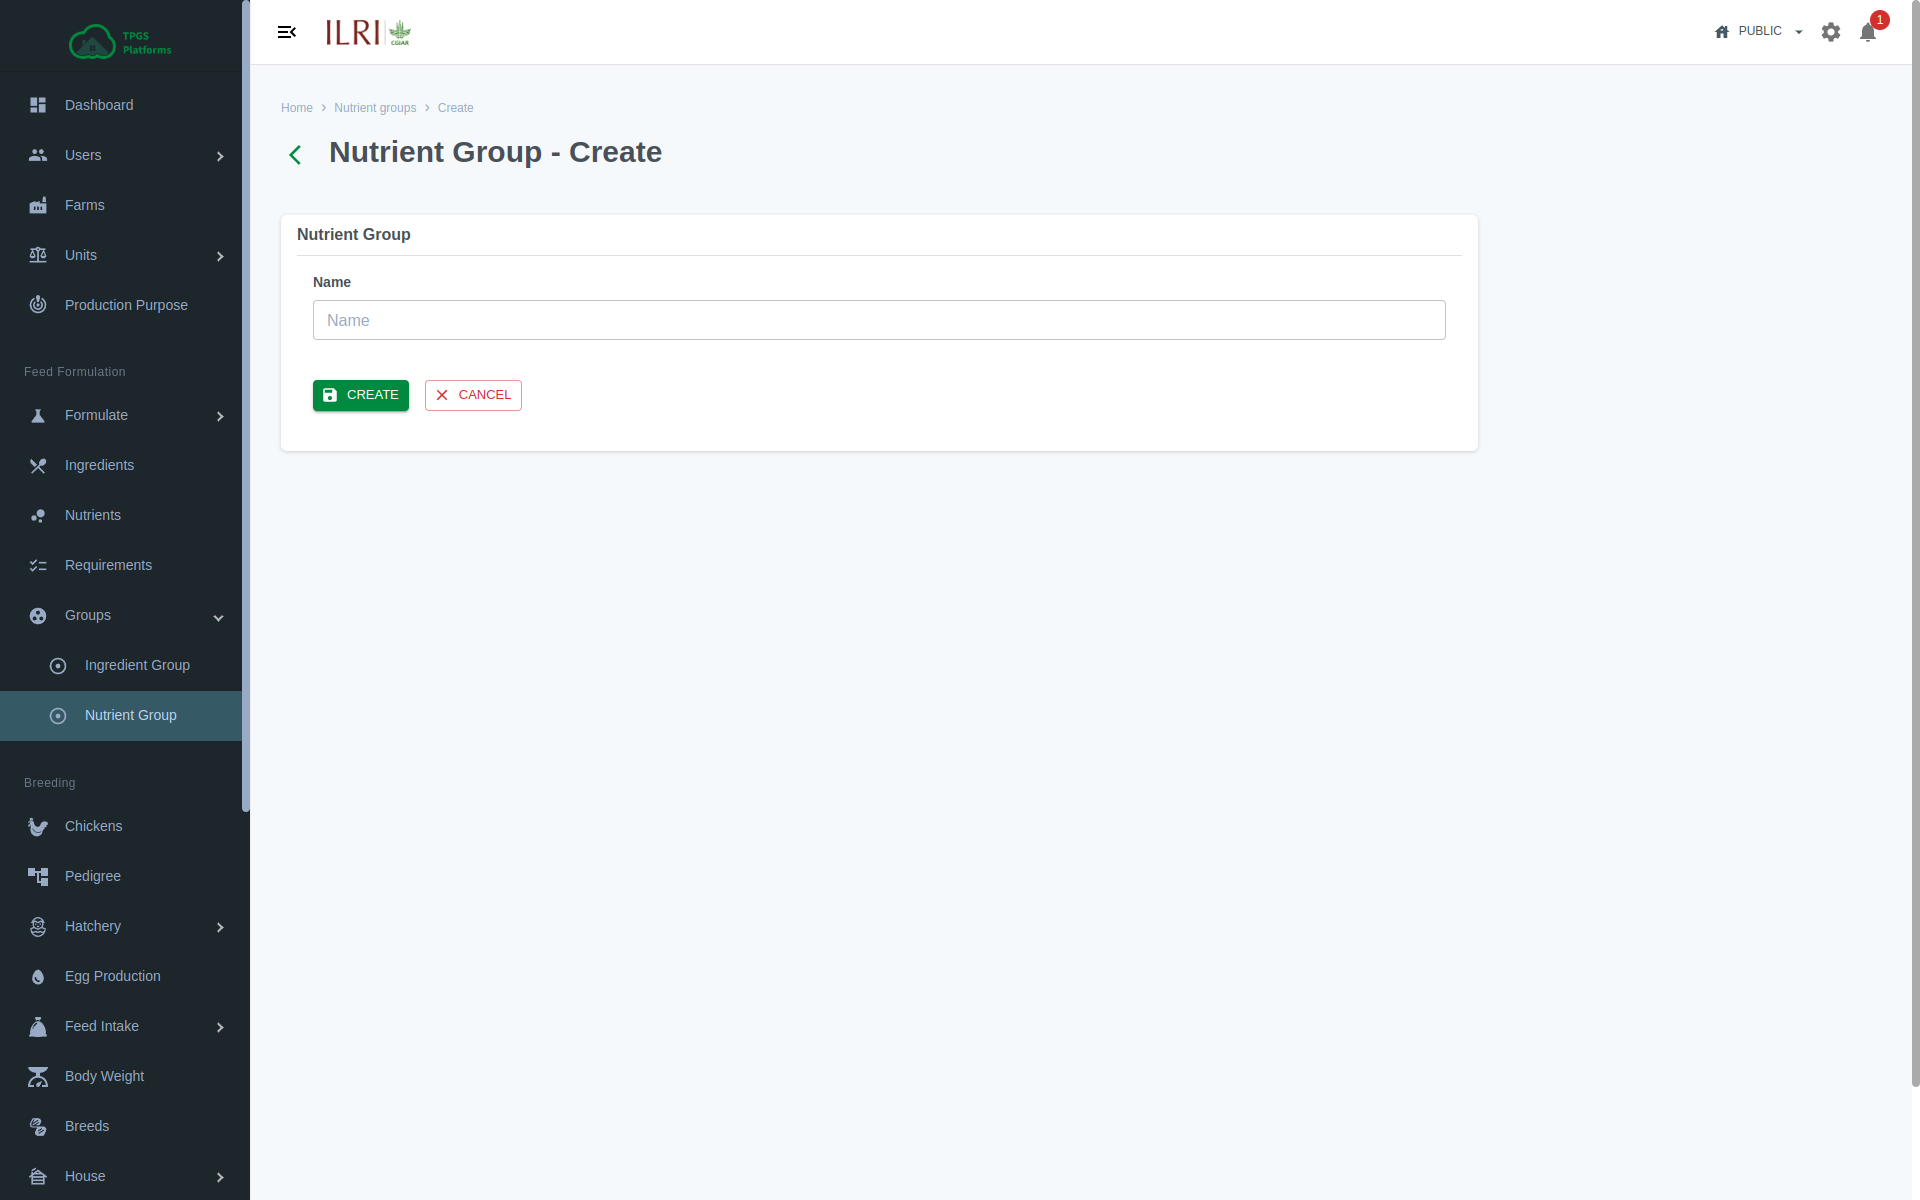
\includegraphics[width=15cm]{screenshots/nutrient_group_create_page.png}
  	\caption{Create new Nutrient Group}
  	\label{fig:nutrient_group_create_page}
\end{figure}
And click \textcolor{ForestGreen}{"CREATE"}, you will be redirect to  \hyperref[sec:nutrient_group_list]{Nutrient List section \ref{sec:nutrient_group_list}}

\subsection{Edit Nutrient Group}\label{sec:nutrient_group_edit}
\setcounter{stepcounter}{1}
\paragraph{\arabic{stepcounter}.}Go to the Nutrient Group \hyperref[sec:nutrient_group_list]{Refer to Section \ref{sec:nutrient_group_list}}, then click on Pencil icon and it will redirect to the \hyperref[fig:nutrient_group_edit_page]{Figure \ref{fig:nutrient_group_edit_page}}.
\begin{figure}[h!]
  	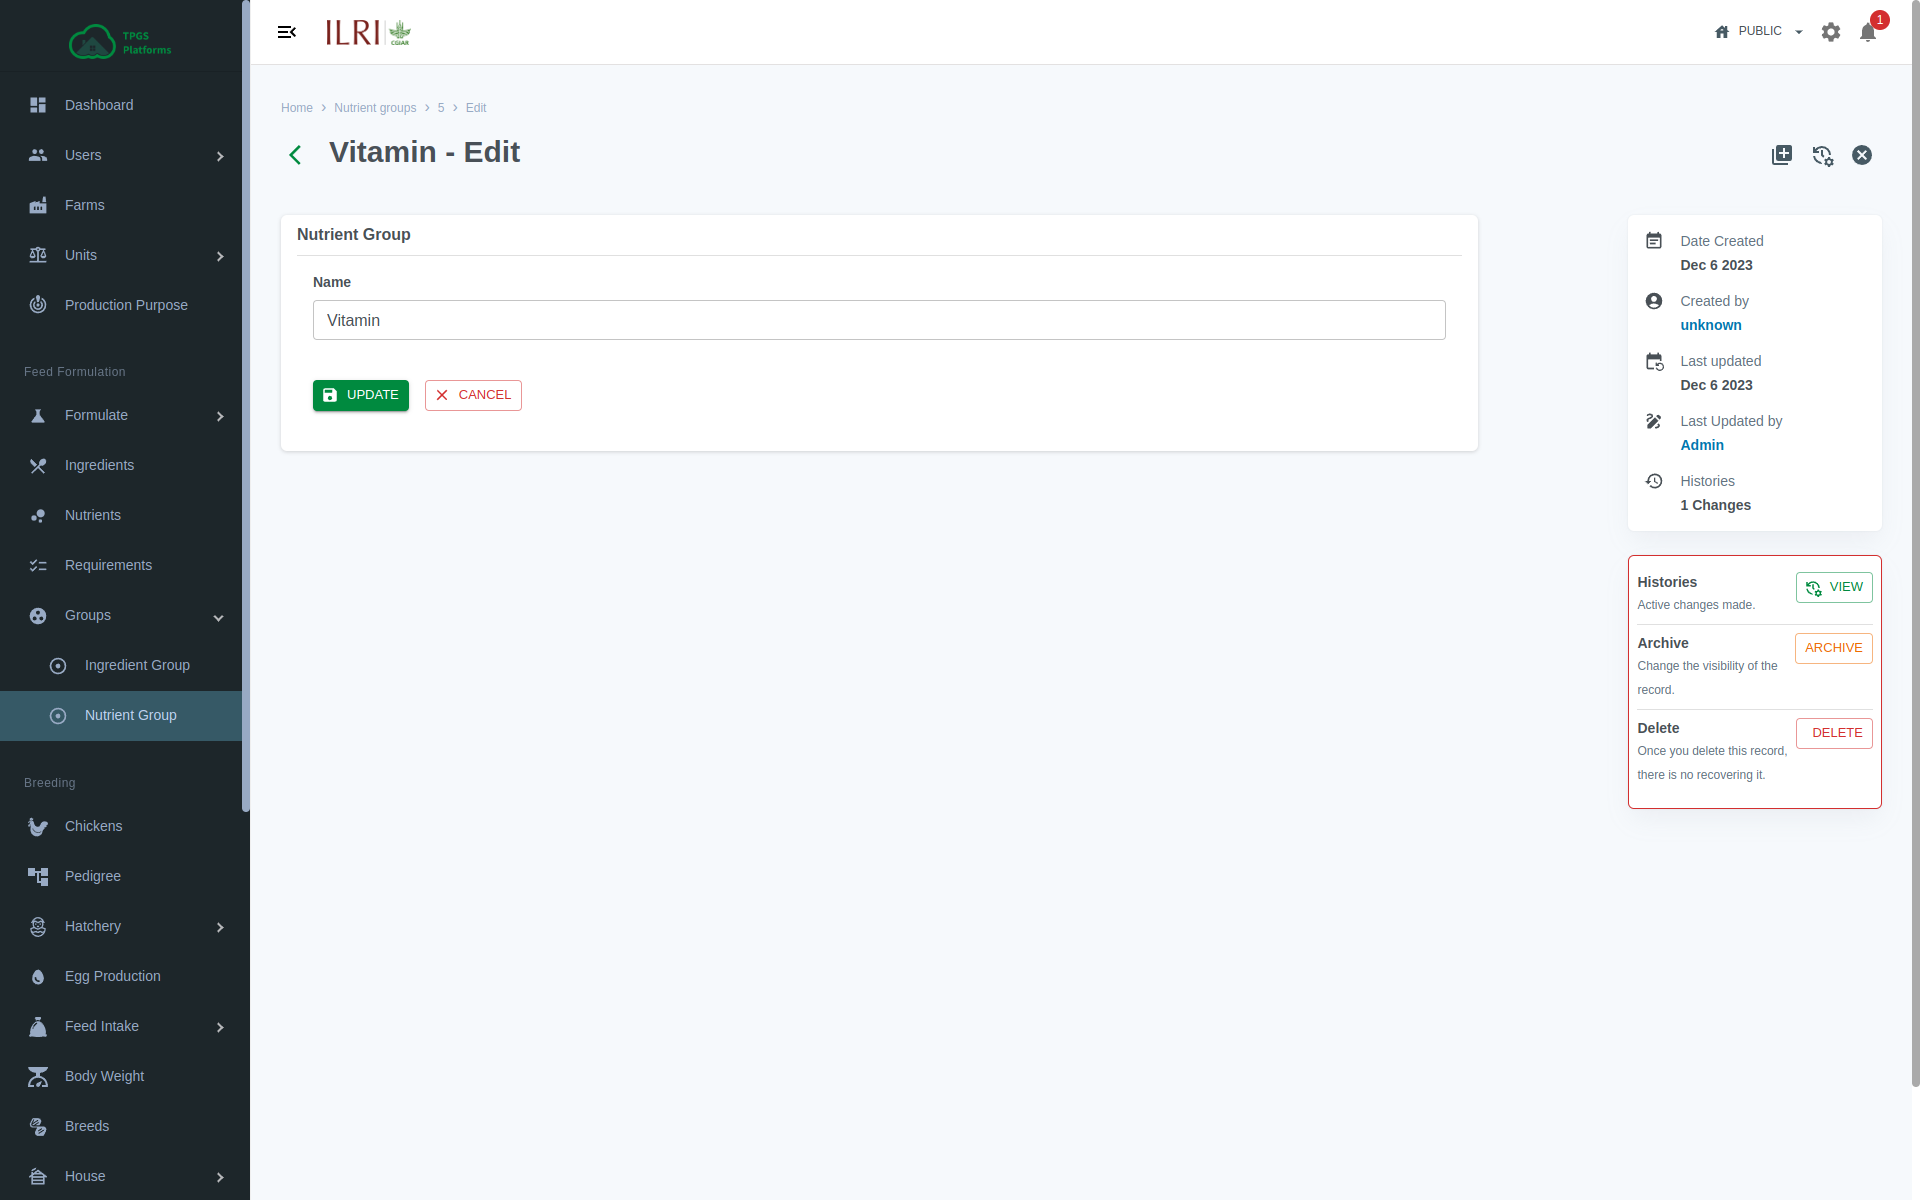
\includegraphics[width=15cm]{screenshots/nutrient_group_edit_page.png}
  	\caption{Edit Nutrient Group}
  	\label{fig:nutrient_group_edit_page}
\end{figure}

\subsection{Delete Nutrient Group}
\setcounter{stepcounter}{1}
\paragraph{\arabic{stepcounter}.}Go to the edit Nutrient Group \hyperref[sec:nutrient_group_edit]{Refer to Section \ref{sec:nutrient_group_edit}}.

\paragraph{\arabic{stepcounter}.}To archive the record click on \textcolor{ForestGreen}{"Archive"}. If you want to bring back the record/unarchive follow the step under \hyperref[sec:nutrient_group_list_archived]{Section  \ref{sec:nutrient_group_list_archived}}, and click on \textcolor{ForestGreen}{"UnArchive"}


\paragraph{\arabic{stepcounter}.}To permanently delete the record click on \textcolor{ForestGreen}{"Delete"}.

\begin{figure}[h!]
  	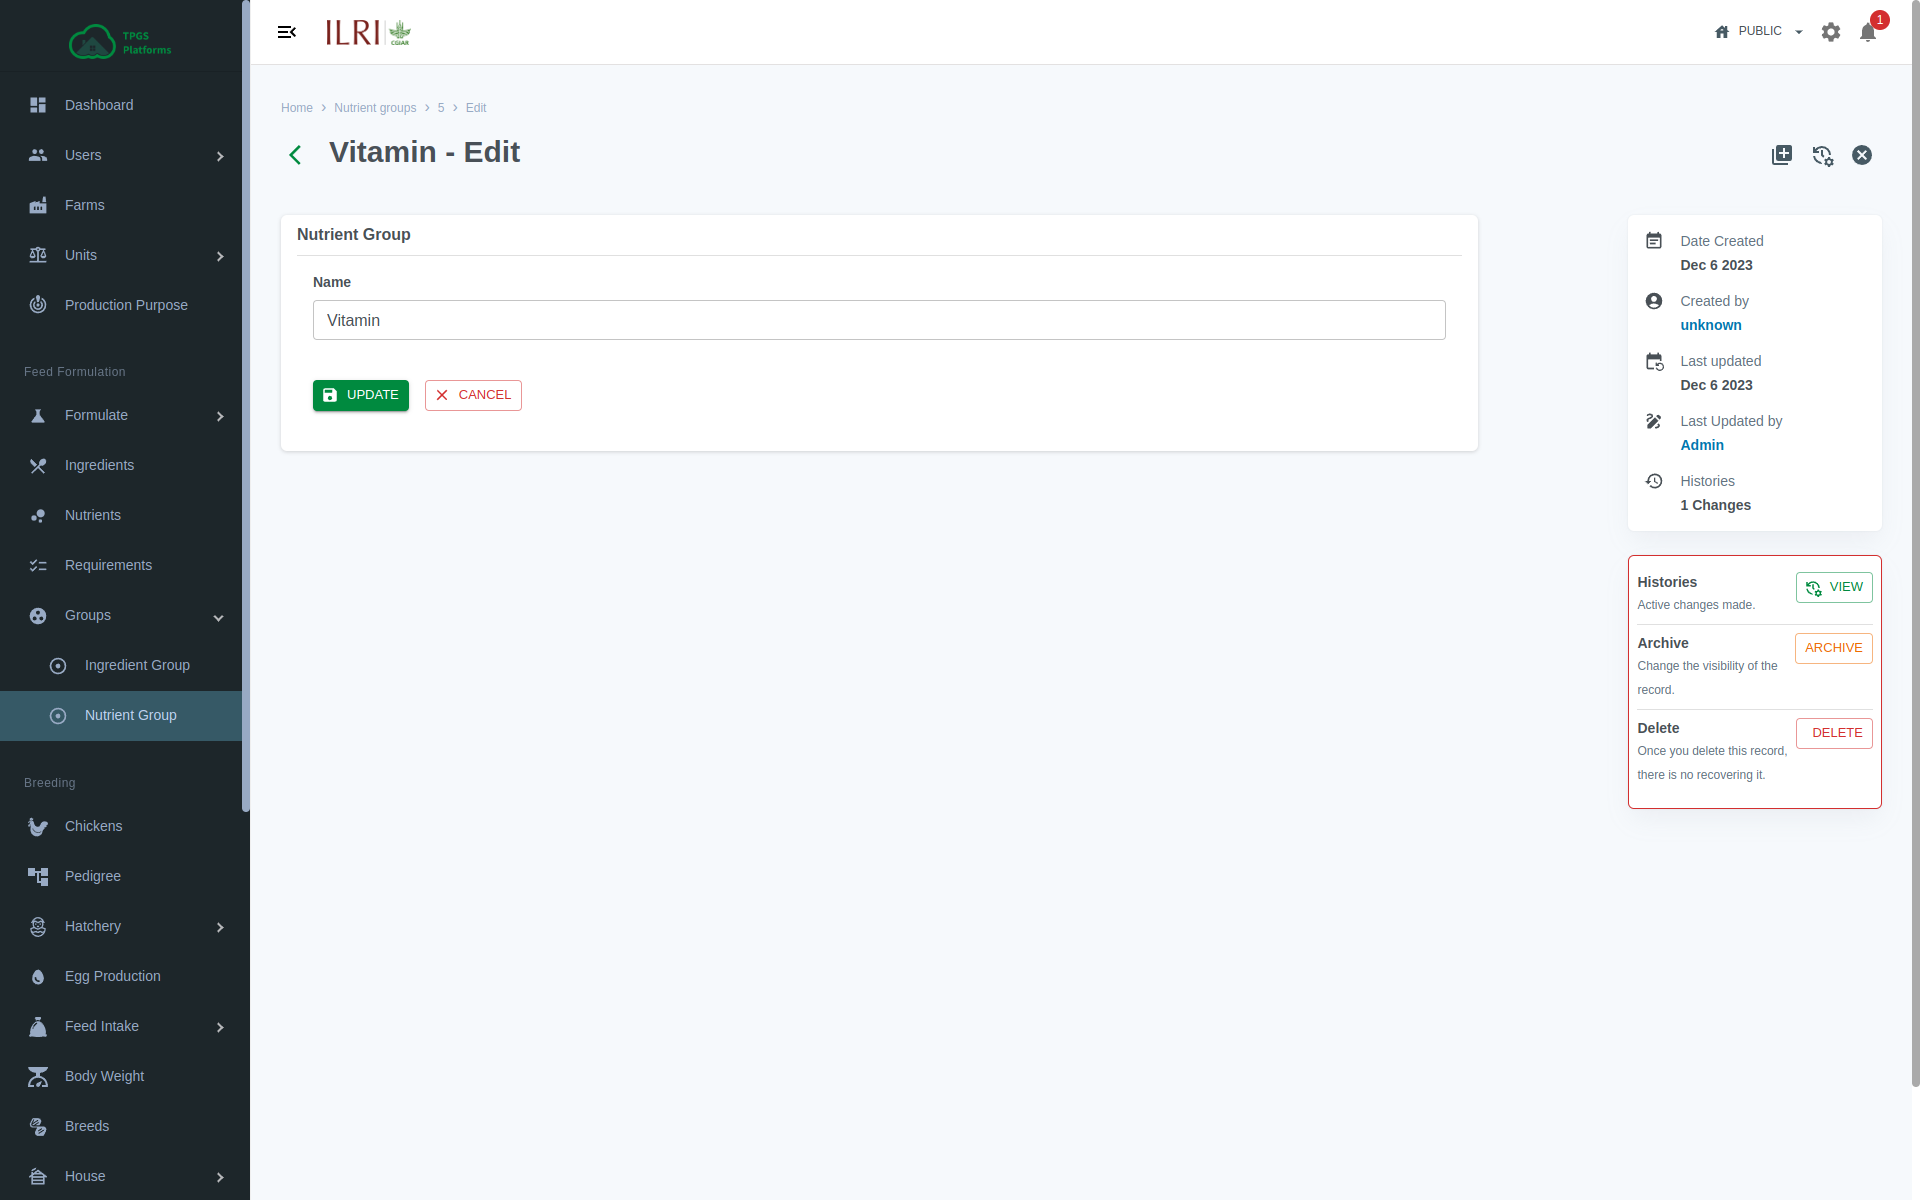
\includegraphics[width=15cm]{screenshots/nutrient_group_edit_page.png}
  	\caption{Edit Nutrient Group}
  	\label{fig:nutrient_group_edit_page}
\end{figure}

\section{Invitation}

\subsection{View Invitations List}
\subsection{Invite User}
\subsection{Resend Invitation}
\subsection{Remove Invitation}

\section{Users}

\subsection{View Users List}
\subsection{Edit User}
\subsection{Deactivate/Activate User's Account}
\subsection{Delete User}
Danger

\section{Settings}
\subsection{Change Password}


\newpage
\section{Nutrient Groups}\label{sec:nutrient_group}

\subsection{View Nutrient Group List}\label{sec:nutrient_group_list}
\setcounter{stepcounter}{1}
\paragraph{\arabic{stepcounter}.}Expand \textcolor{ForestGreen}{"Group"} menu and click on \textcolor{ForestGreen}{"Nutrient Group"}
\begin{figure}[h!]
  	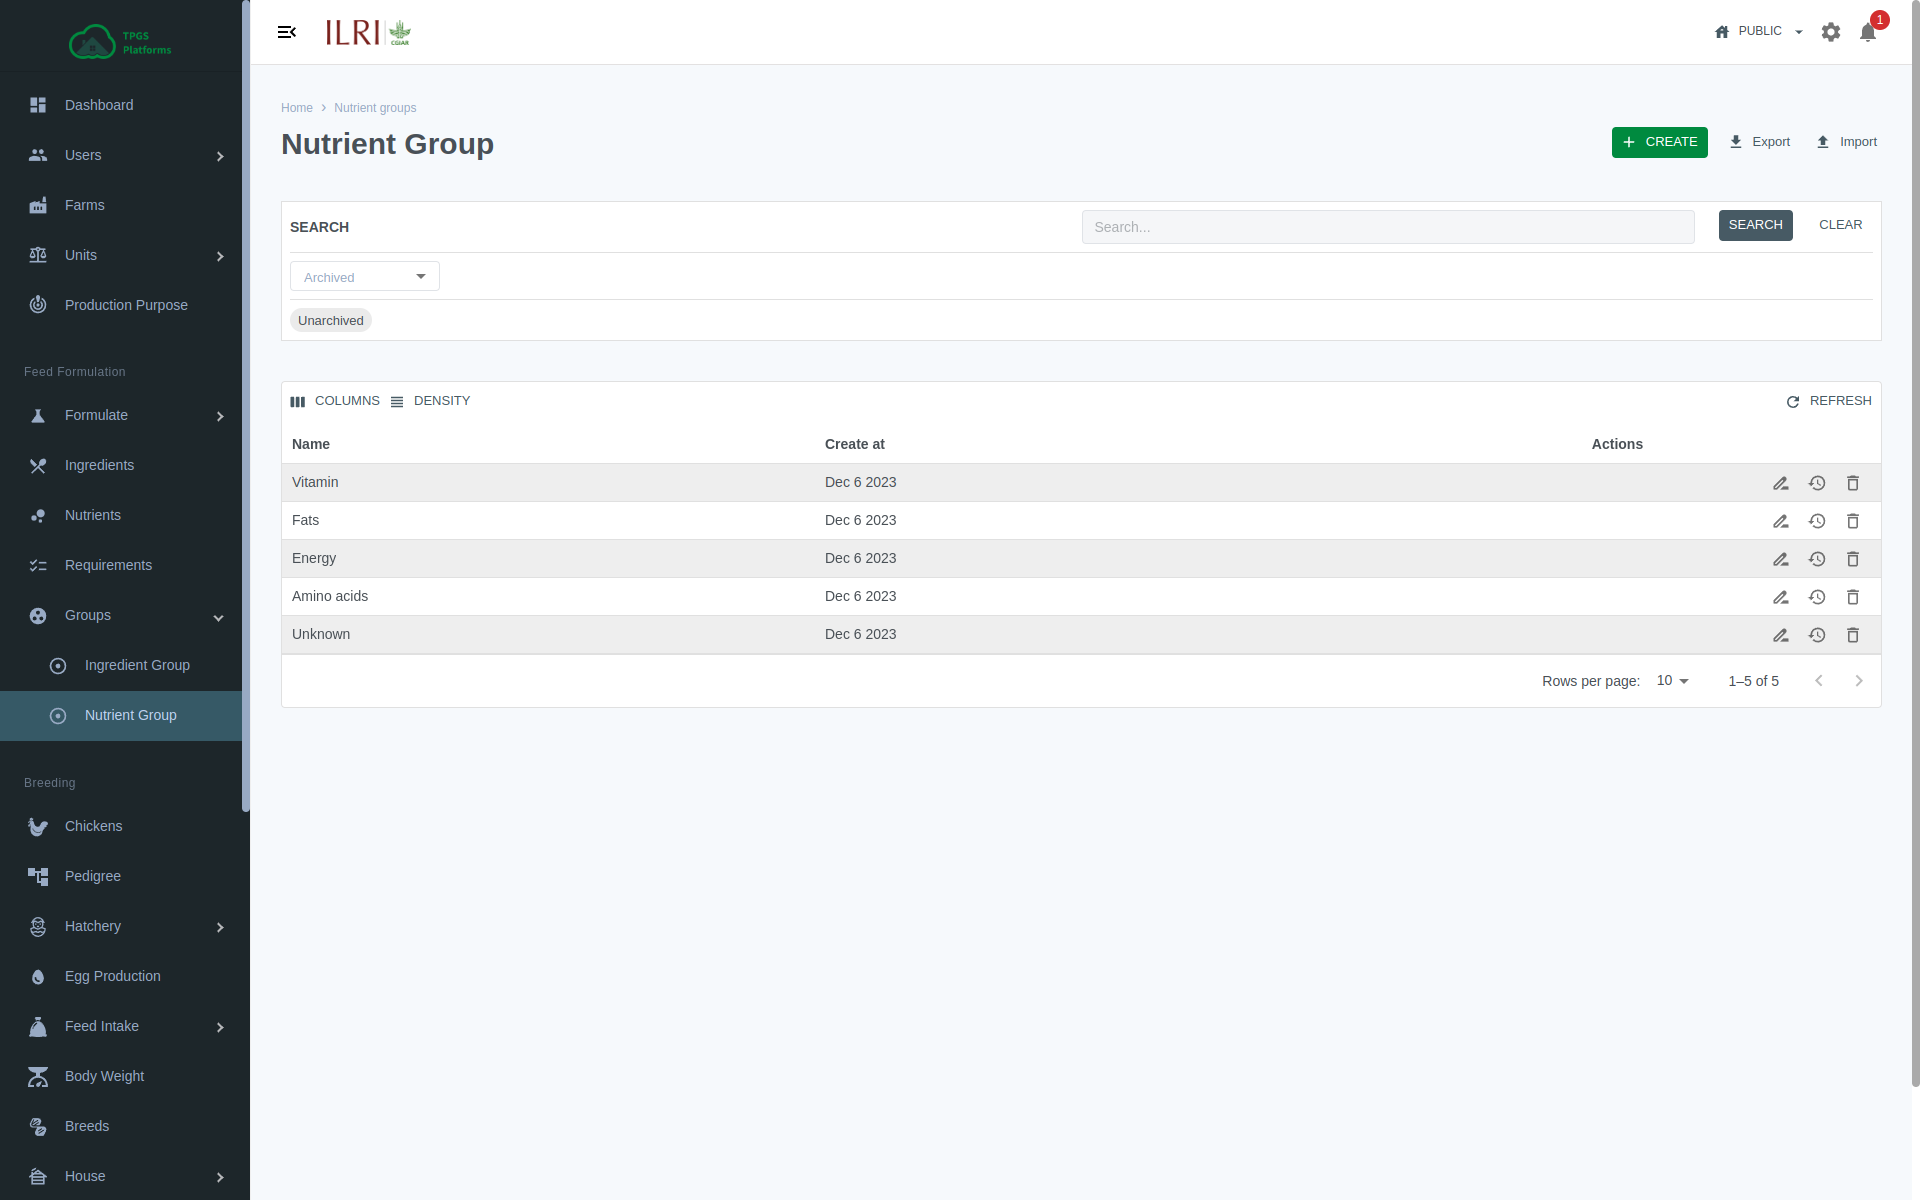
\includegraphics[width=15cm]{screenshots/nutrient_group_list_page.png}
  	\caption{Nutrient Group List}
  	\label{fig:nutrient_group_list_page}
\end{figure}

\subsection{Archive Records}\label{sec:nutrient_group_list_archived}
\setcounter{stepcounter}{1}
\paragraph{\arabic{stepcounter}.}On filter section filter the records by archive.

\subsection{Create new Nutrient Group}\label{sec:nutrient_group_create}
\setcounter{stepcounter}{1}
\paragraph{\arabic{stepcounter}.}To create new nutrient group click on \textcolor{ForestGreen}{"Create"} \hyperref[fig:nutrient_group_list_page]{Refer from nutrient list Figure \ref{fig:nutrient_group_list_page}}
\begin{figure}[h!]
  	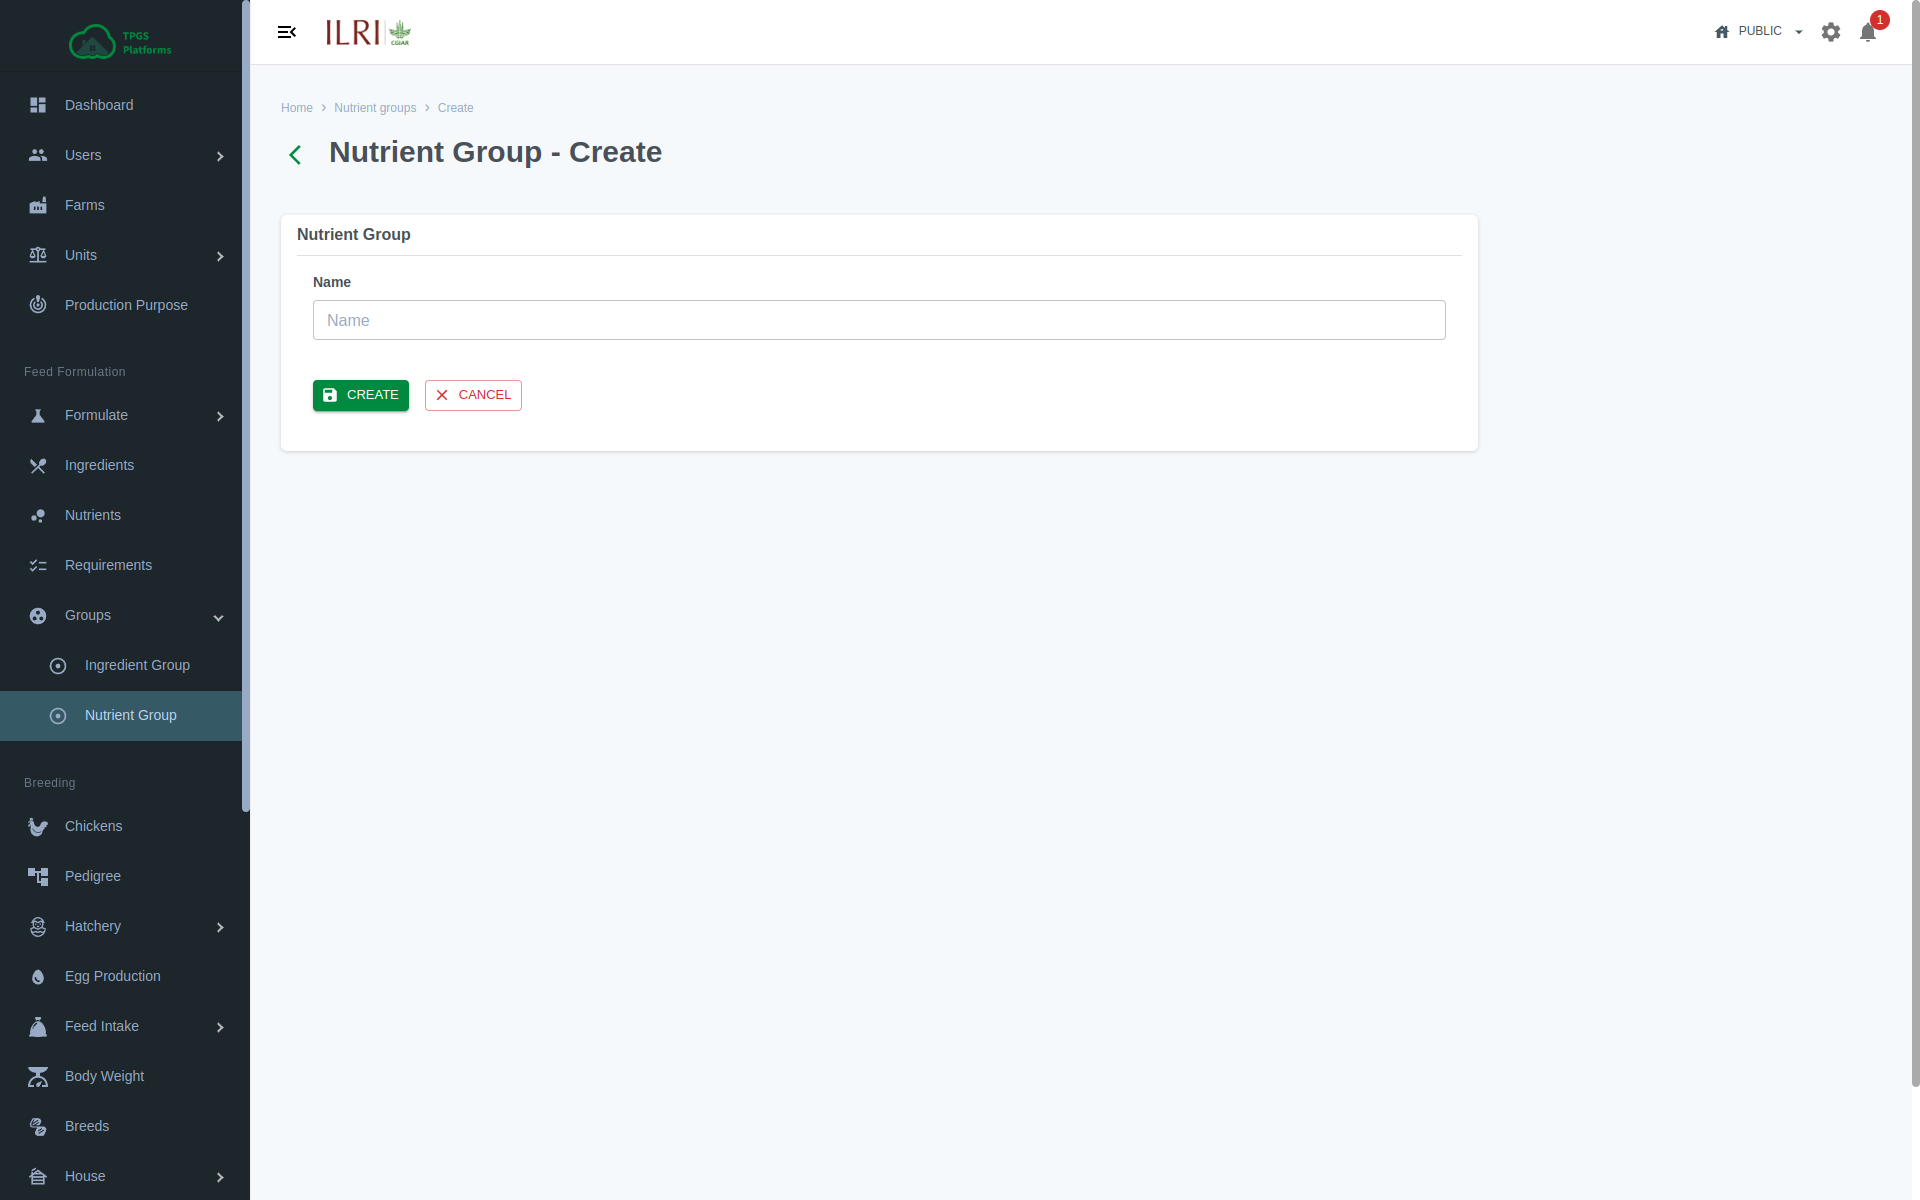
\includegraphics[width=15cm]{screenshots/nutrient_group_create_page.png}
  	\caption{Create new Nutrient Group}
  	\label{fig:nutrient_group_create_page}
\end{figure}
And click \textcolor{ForestGreen}{"CREATE"}, you will be redirect to  \hyperref[sec:nutrient_group_list]{Nutrient List section \ref{sec:nutrient_group_list}}

\subsection{Edit Nutrient Group}\label{sec:nutrient_group_edit}
\setcounter{stepcounter}{1}
\paragraph{\arabic{stepcounter}.}Go to the Nutrient Group \hyperref[sec:nutrient_group_list]{Refer to Section \ref{sec:nutrient_group_list}}, then click on Pencil icon and it will redirect to the \hyperref[fig:nutrient_group_edit_page]{Figure \ref{fig:nutrient_group_edit_page}}.
\begin{figure}[h!]
  	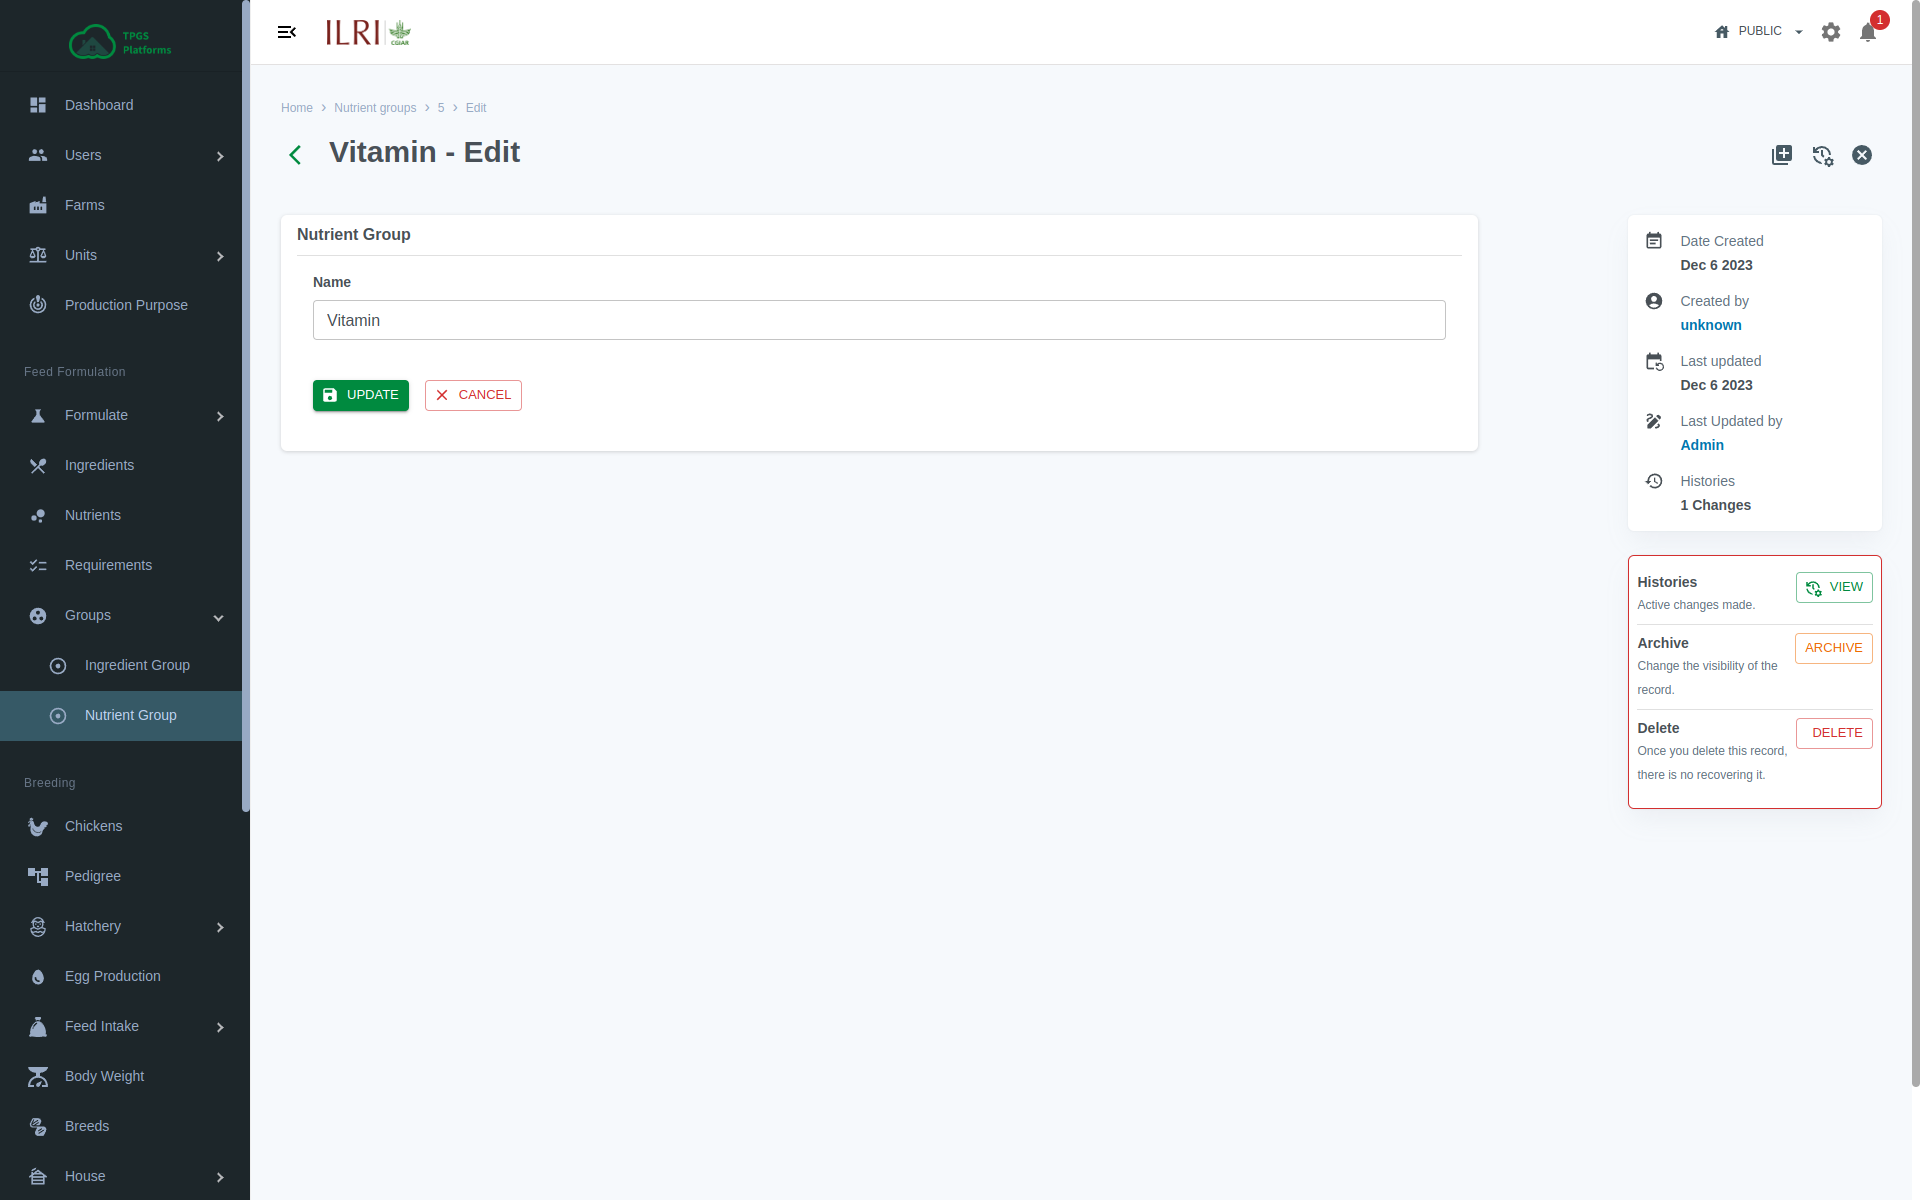
\includegraphics[width=15cm]{screenshots/nutrient_group_edit_page.png}
  	\caption{Edit Nutrient Group}
  	\label{fig:nutrient_group_edit_page}
\end{figure}

\subsection{Delete Nutrient Group}
\setcounter{stepcounter}{1}
\paragraph{\arabic{stepcounter}.}Go to the edit Nutrient Group \hyperref[sec:nutrient_group_edit]{Refer to Section \ref{sec:nutrient_group_edit}}.

\paragraph{\arabic{stepcounter}.}To archive the record click on \textcolor{ForestGreen}{"Archive"}. If you want to bring back the record/unarchive follow the step under \hyperref[sec:nutrient_group_list_archived]{Section  \ref{sec:nutrient_group_list_archived}}, and click on \textcolor{ForestGreen}{"UnArchive"}


\paragraph{\arabic{stepcounter}.}To permanently delete the record click on \textcolor{ForestGreen}{"Delete"}.

\begin{figure}[h!]
  	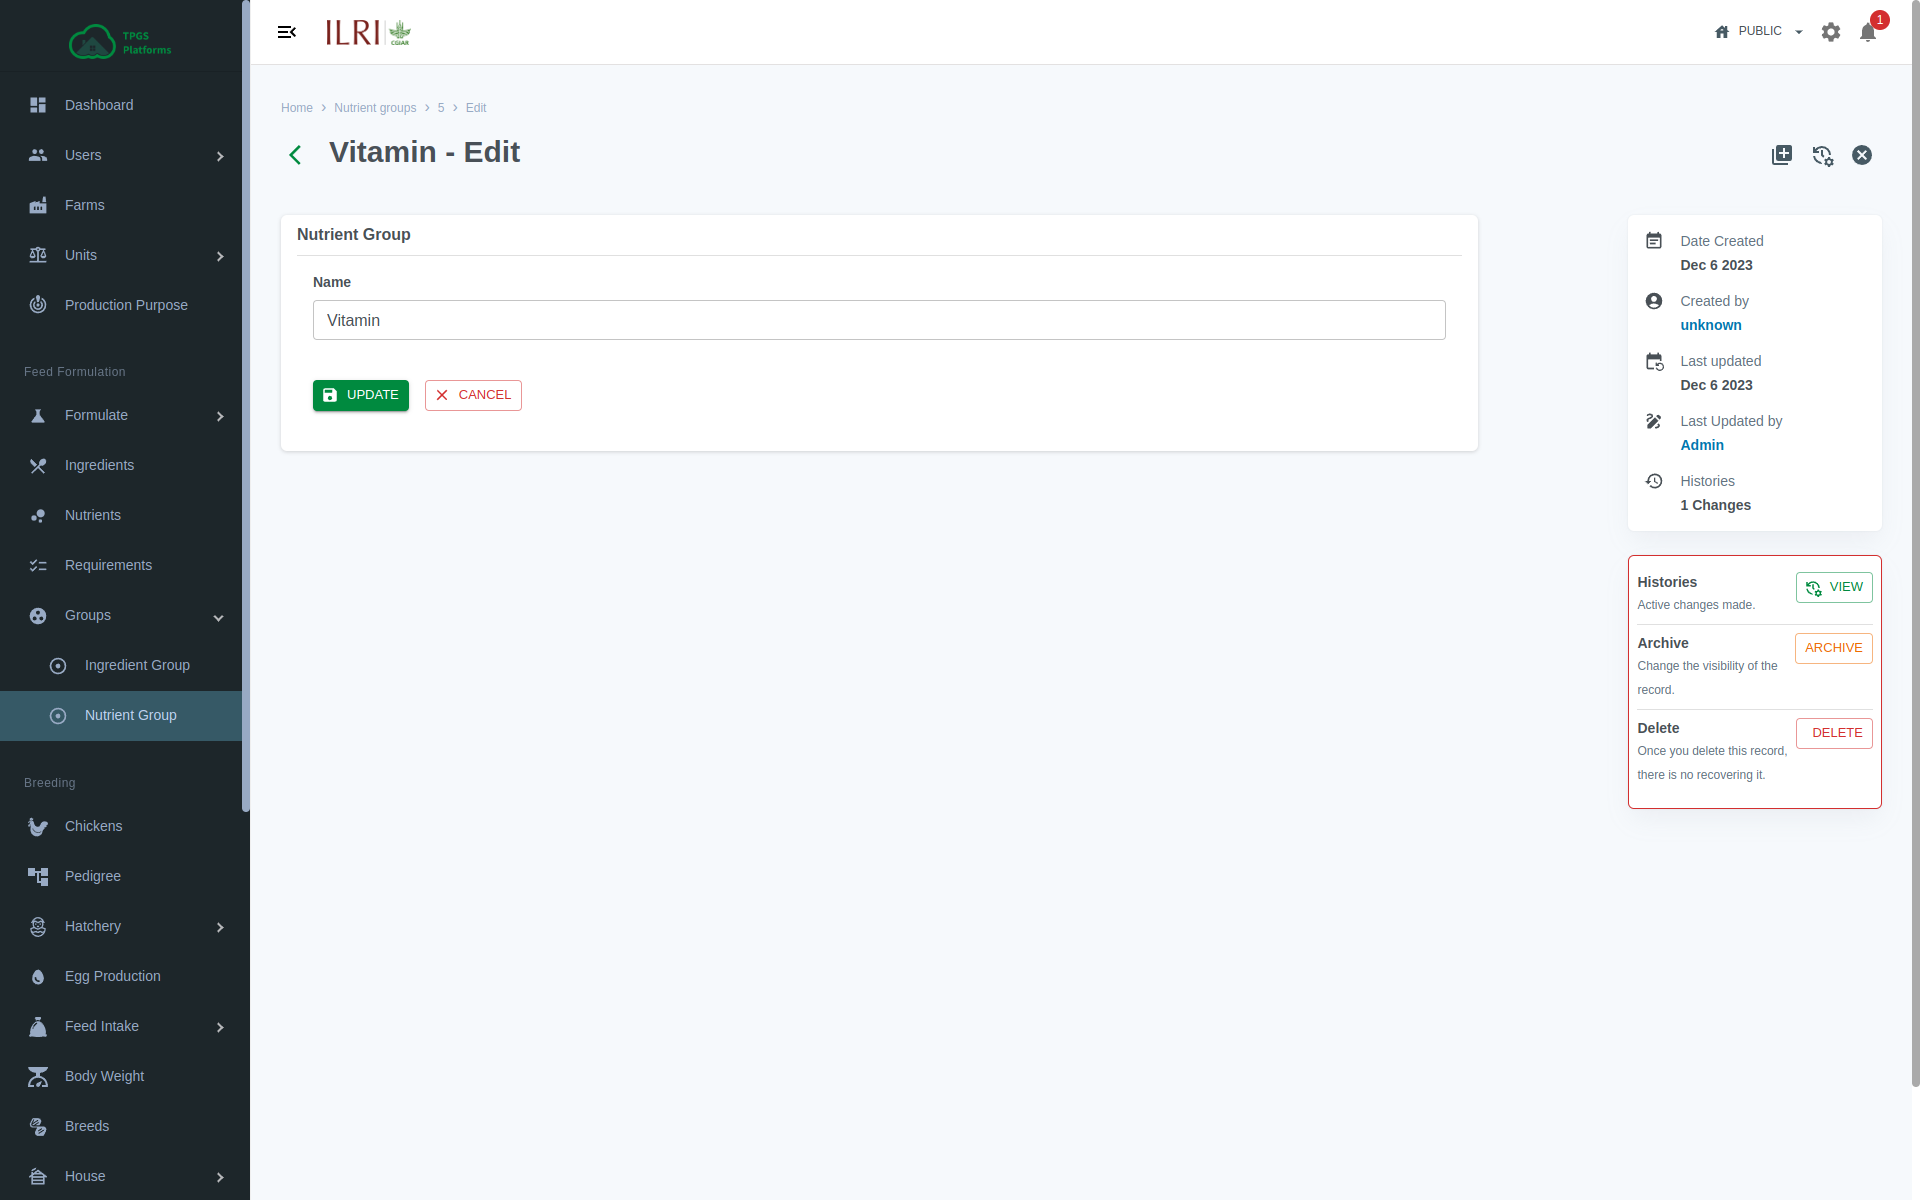
\includegraphics[width=15cm]{screenshots/nutrient_group_edit_page.png}
  	\caption{Edit Nutrient Group}
  	\label{fig:nutrient_group_edit_page}
\end{figure}

\newpage
\section{Nutrient}\label{sec:nutrient}

\subsection{View Nutrient  List}\label{sec:nutrient_list}
\setcounter{stepcounter}{1}
\paragraph{\arabic{stepcounter}.}Expand \textcolor{ForestGreen}{"Group"} menu and click on \textcolor{ForestGreen}{"Nutrient "}
\begin{figure}[h!]
  	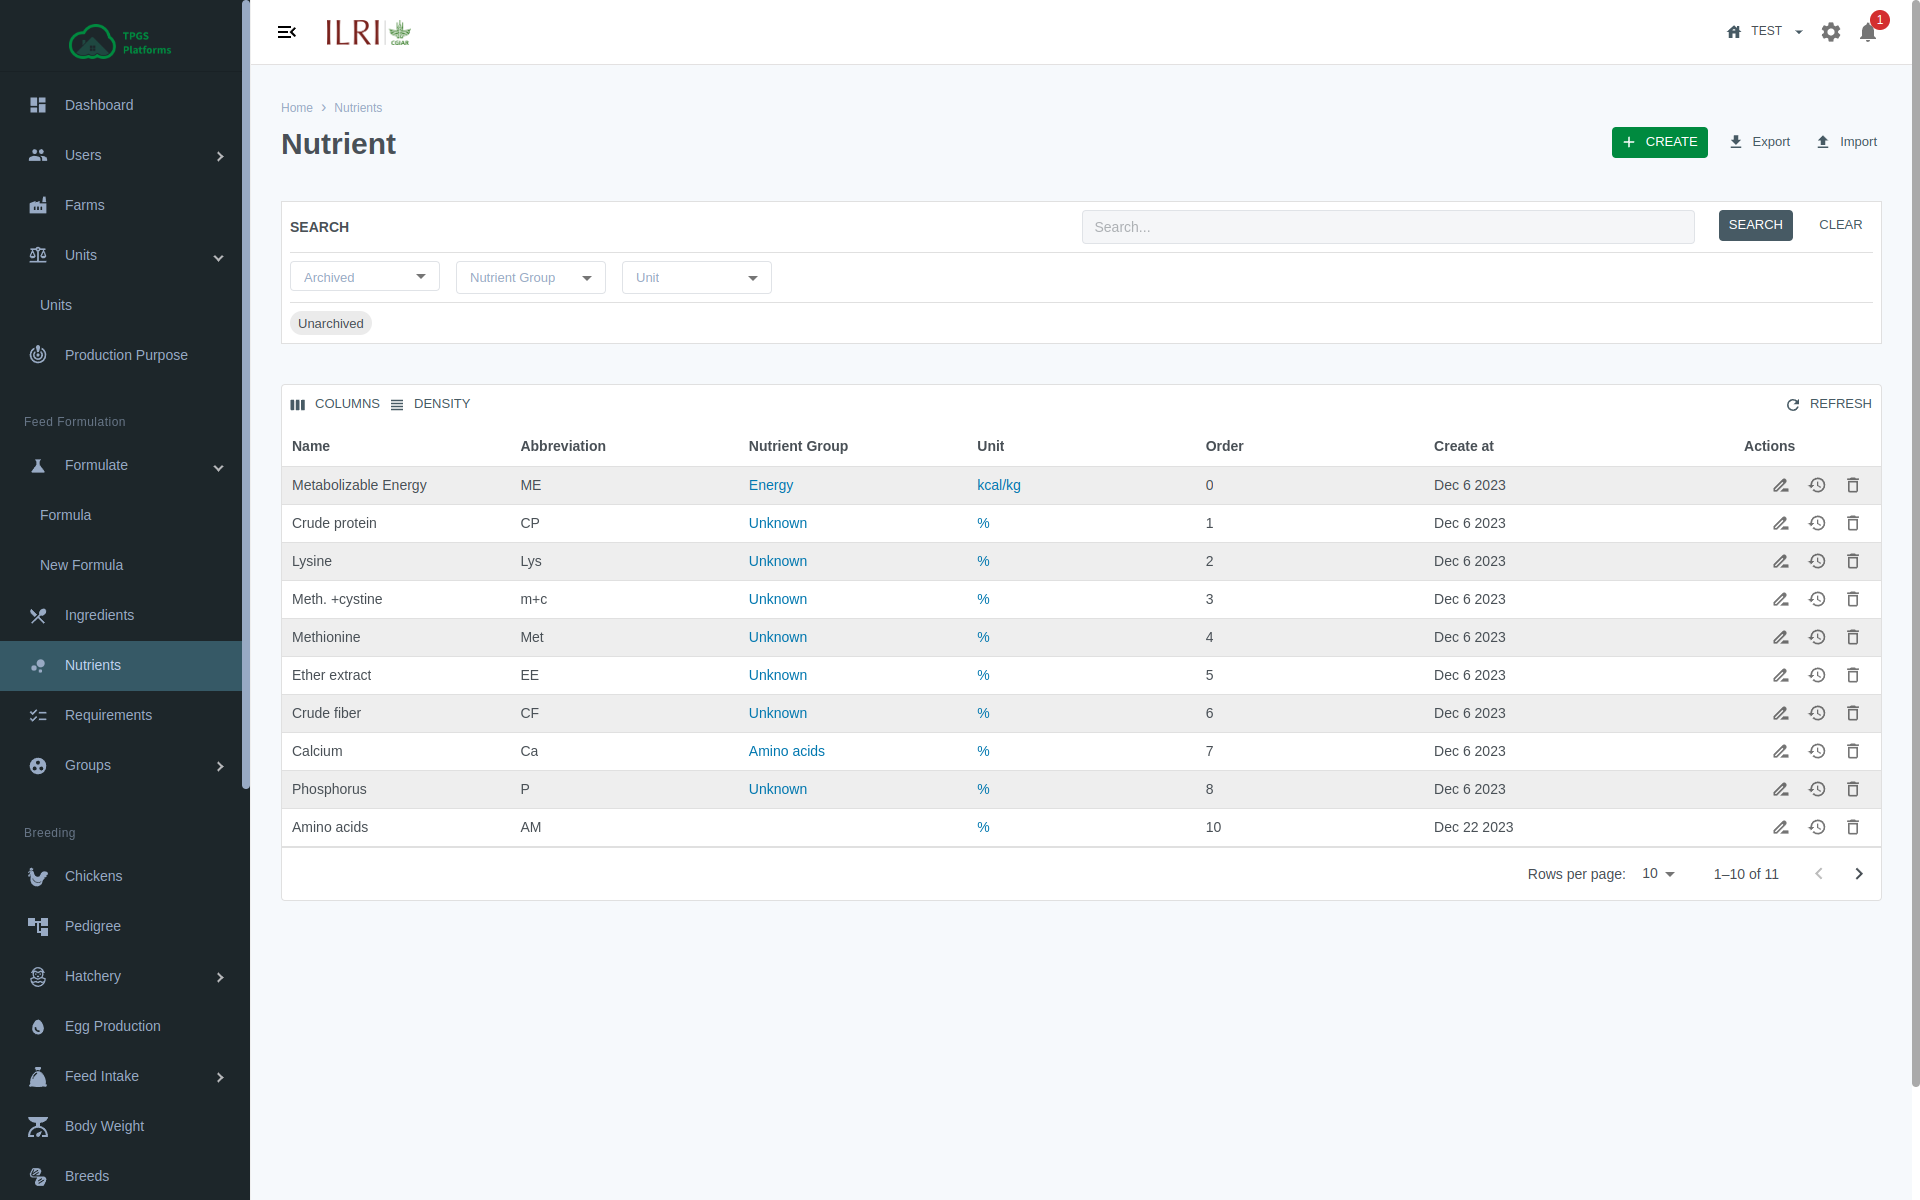
\includegraphics[width=15cm]{screenshots/nutrient_list_page.png}
  	\caption{Nutrient  List}
  	\label{fig:nutrient_list_page}
\end{figure}

\subsection{Archive Records}\label{sec:nutrient_list_archived}
\setcounter{stepcounter}{1}
\paragraph{\arabic{stepcounter}.}On filter section filter the records by archive.

\subsection{Create new Nutrient }\label{sec:nutrient_create}
\setcounter{stepcounter}{1}
\paragraph{\arabic{stepcounter}.}To create new nutrient group click on \textcolor{ForestGreen}{"Create"} \hyperref[fig:nutrient_list_page]{Refer from nutrient list Figure \ref{fig:nutrient_list_page}}
\begin{figure}[h!]
  	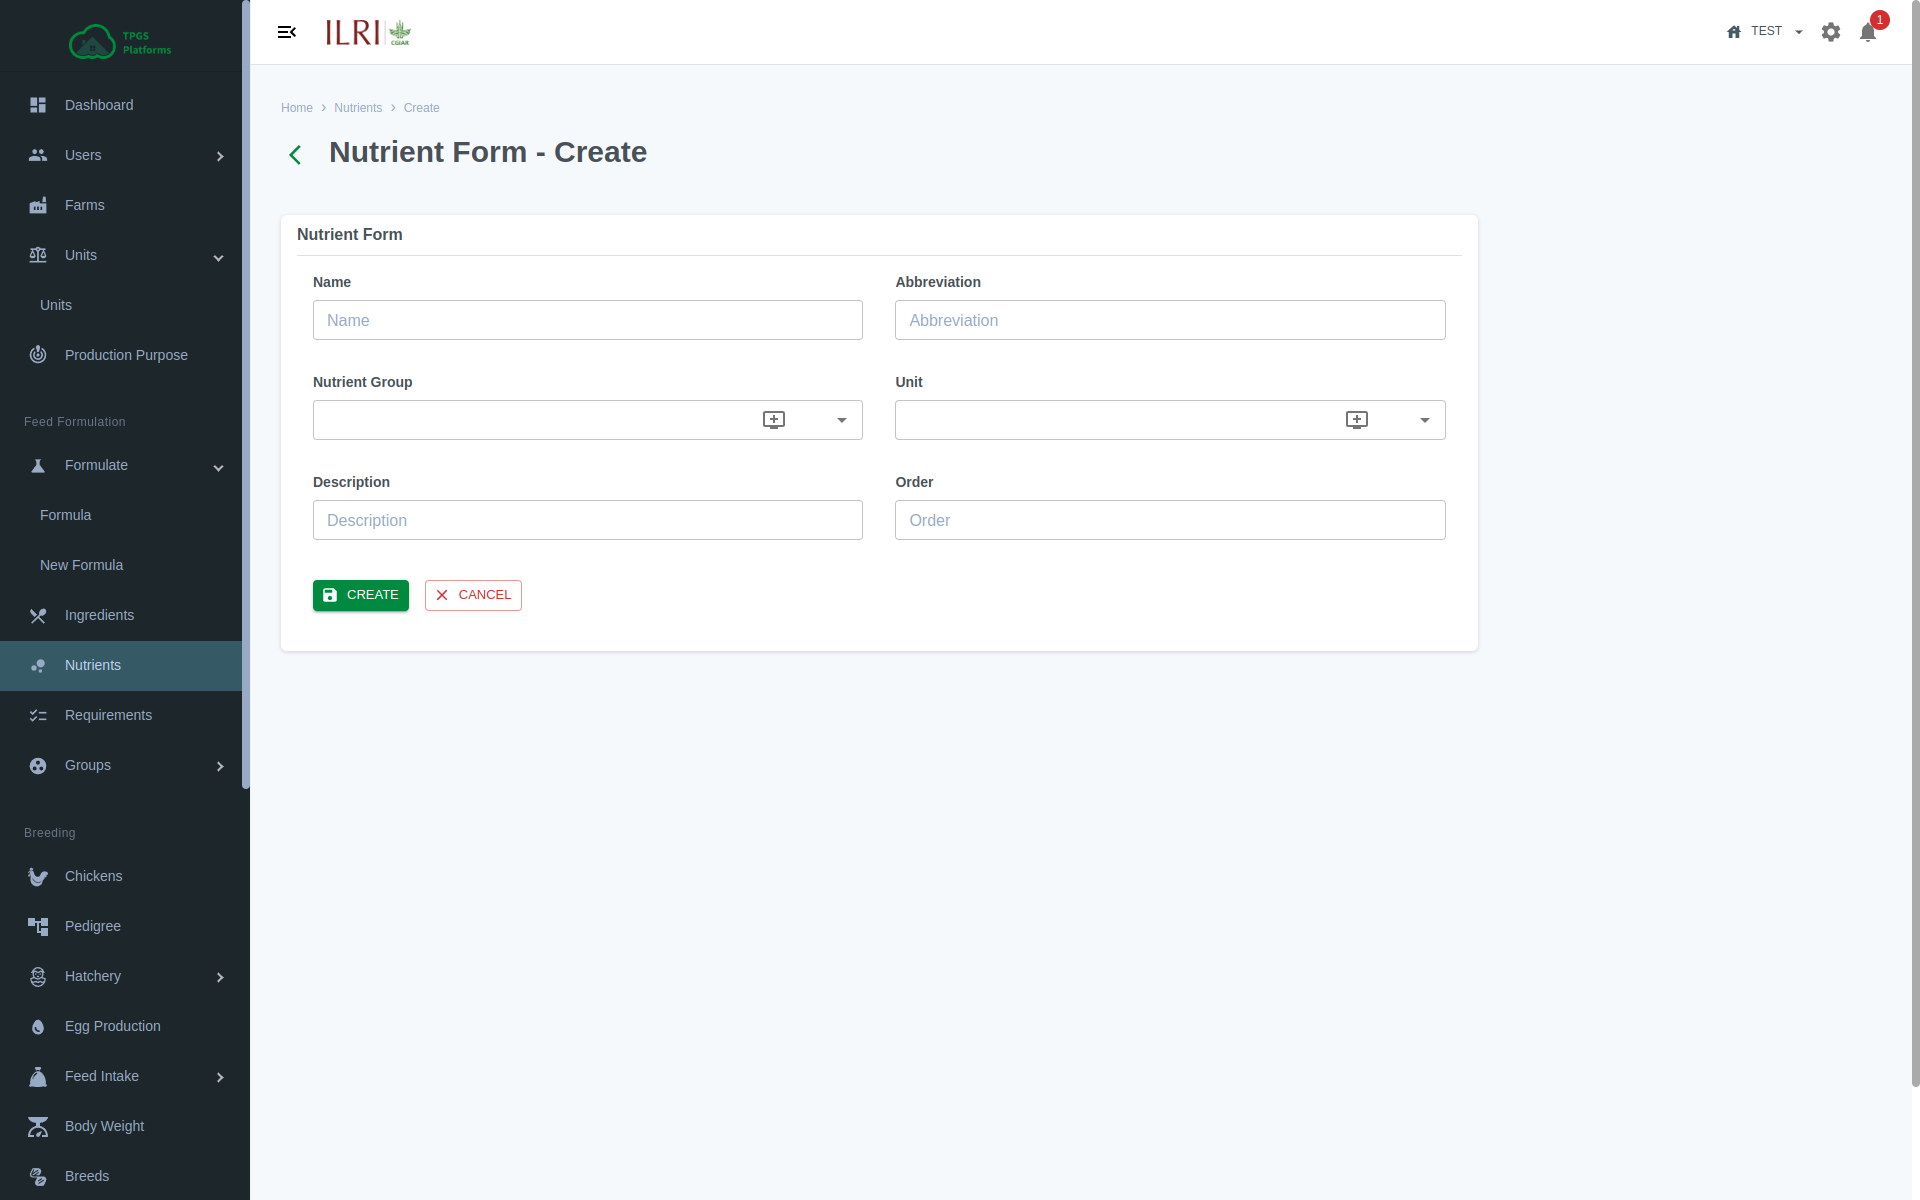
\includegraphics[width=15cm]{screenshots/nutrient_create_page.png}
  	\caption{Create new Nutrient }
  	\label{fig:nutrient_create_page}
\end{figure}
And click \textcolor{ForestGreen}{"CREATE"}, you will be redirect to  \hyperref[sec:nutrient_list]{Nutrient List section \ref{sec:nutrient_list}}

\subsection{Edit Nutrient }\label{sec:nutrient_edit}
\setcounter{stepcounter}{1}
\paragraph{\arabic{stepcounter}.}Go to the Nutrient  \hyperref[sec:nutrient_list]{Refer to Section \ref{sec:nutrient_list}}, then click on Pencil icon and it will redirect to the \hyperref[fig:nutrient_edit_page]{Figure \ref{fig:nutrient_edit_page}}.
\begin{figure}[h!]
  	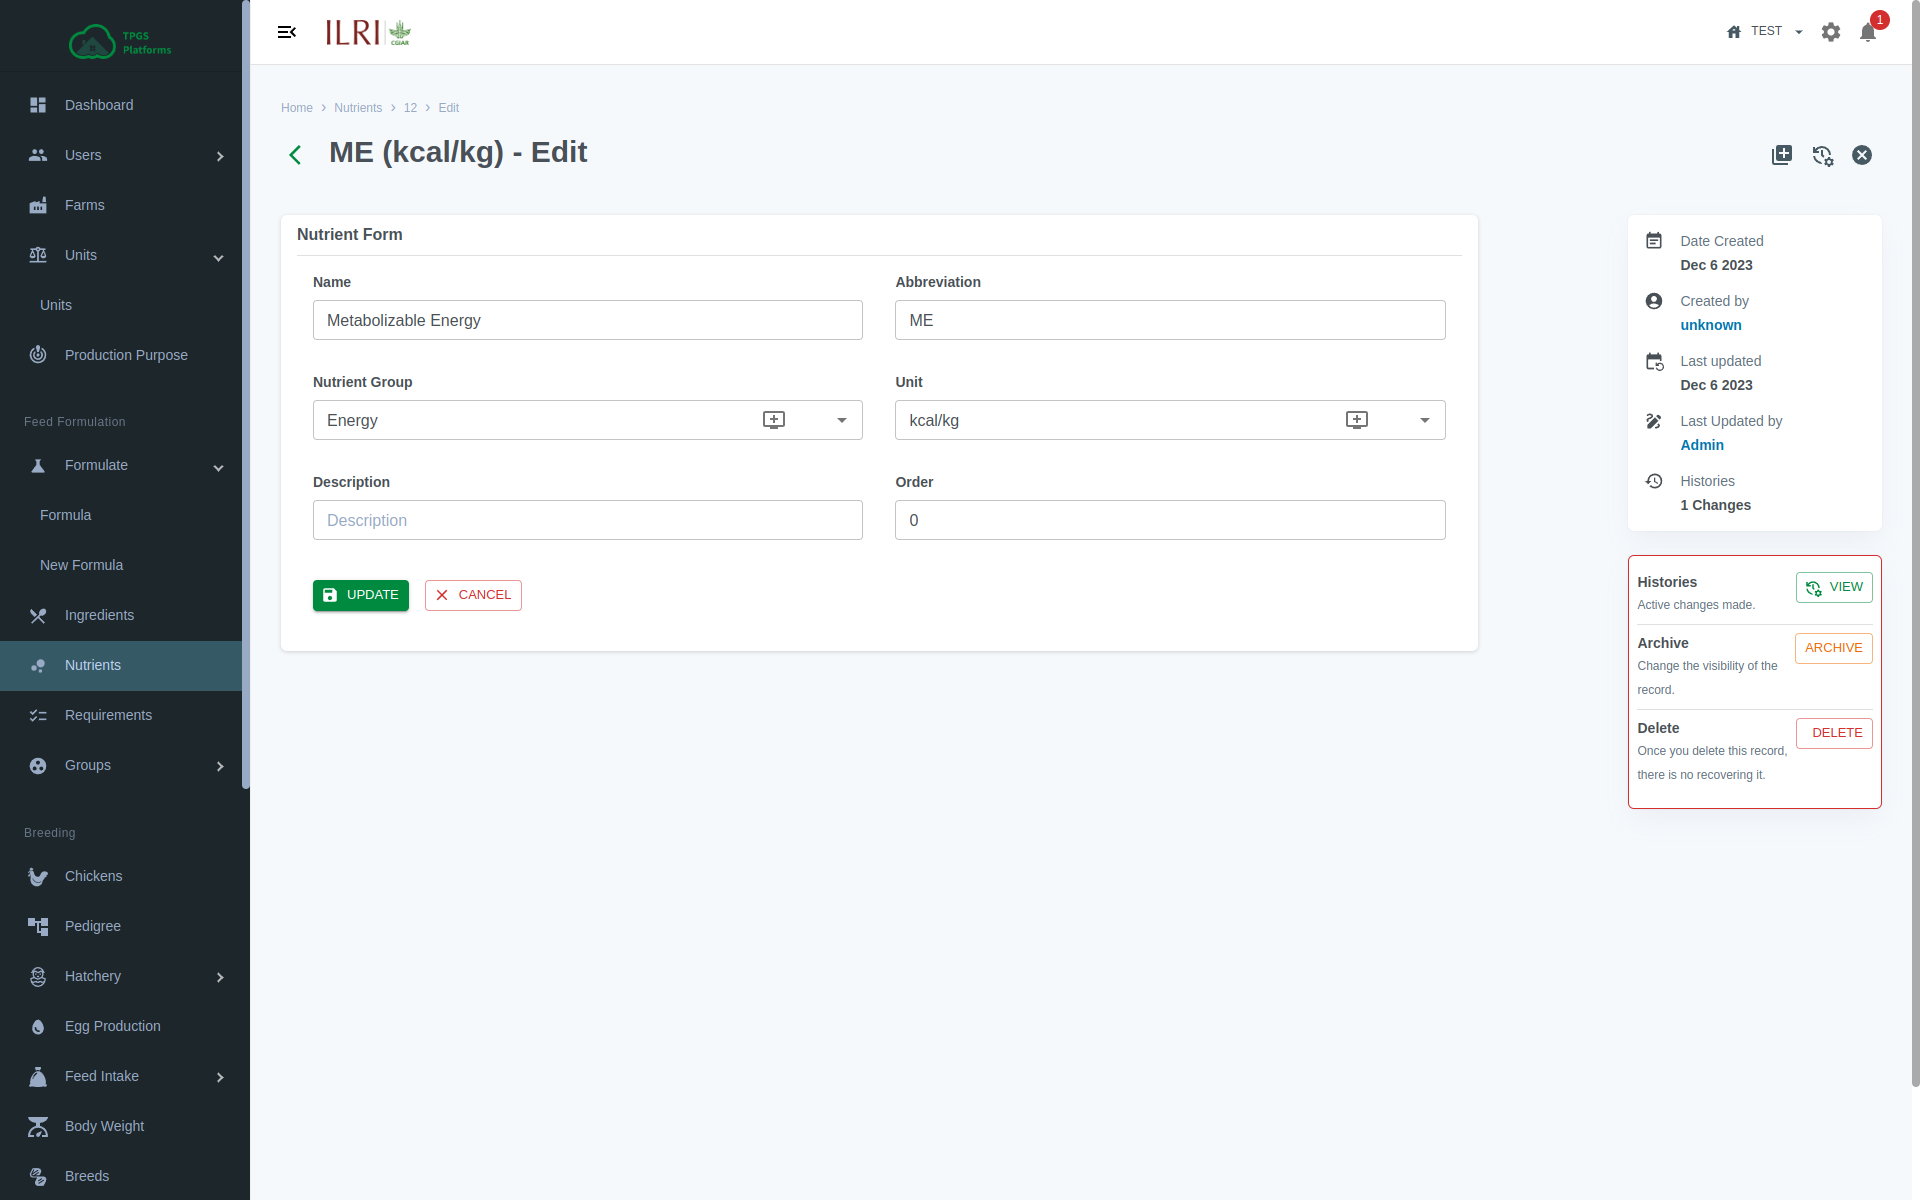
\includegraphics[width=15cm]{screenshots/nutrient_edit_page.png}
  	\caption{Edit Nutrient }
  	\label{fig:nutrient_edit_page}
\end{figure}

\subsection{Delete Nutrient }
\setcounter{stepcounter}{1}
\paragraph{\arabic{stepcounter}.}Go to the edit Nutrient  \hyperref[sec:nutrient_edit]{Refer to Section \ref{sec:nutrient_edit}}.

\paragraph{\arabic{stepcounter}.}To archive the record click on \textcolor{ForestGreen}{"Archive"}. If you want to bring back the record/unarchive follow the step under \hyperref[sec:nutrient_list_archived]{Section  \ref{sec:nutrient_list_archived}}, and click on \textcolor{ForestGreen}{"UnArchive"}


\paragraph{\arabic{stepcounter}.}To permanently delete the record click on \textcolor{ForestGreen}{"Delete"}.

\begin{figure}[h!]
  	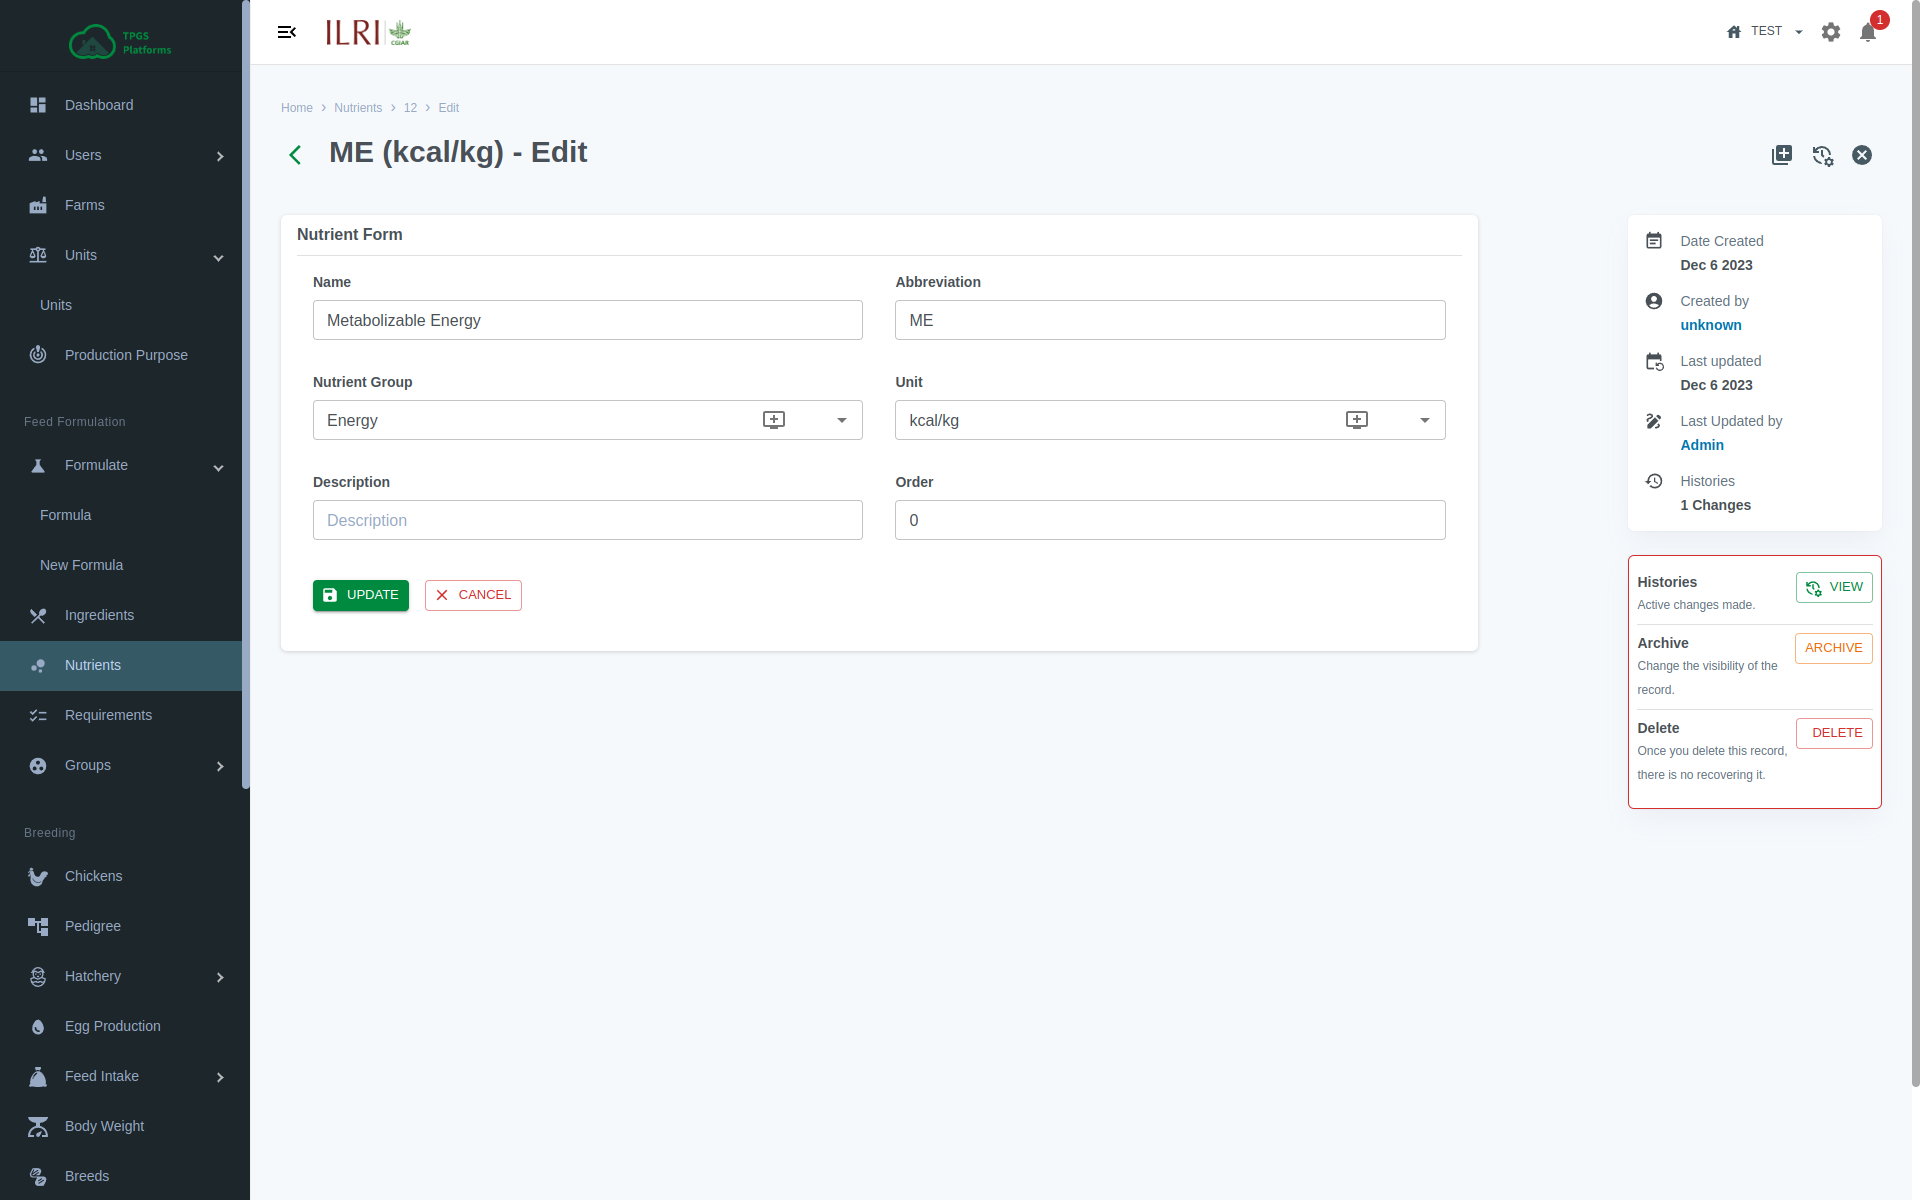
\includegraphics[width=15cm]{screenshots/nutrient_edit_page.png}
  	\caption{Edit Nutrient }
  	\label{fig:nutrient_edit_page}
\end{figure}

\section{Ingredient Groups}

\section{Ingredients}

\section{Requirement}

\section{Ration Formulation}


\newpage
\section{Contact Info}\label{sec:contact_info}

support email address example@example.com

\newpage
\section{Reference}
\printbibliography[title={References}]

\end{document}